% KLTN template (HCMUS) adapted for the HSGE thesis — English report.
% Build order: clean aux files, then PDFLATEX > BIBTEX > PDFLATEX > PDFLATEX.
%   rm -f *.aux *.bbl *.blg *.log *.out *.toc *.lof *.lot *.run.xml *-blx.bib
%   rm -f Chapter*/*.aux Appendix/*.aux
%   pdflatex -interaction=nonstopmode main.tex && bibtex main
%   pdflatex -interaction=nonstopmode main.tex && pdflatex -interaction=nonstopmode main.tex

\documentclass[oneside,a4paper,14pt]{extreport}

% Vietnamese support (needed for the cover page and names)
\usepackage[T5]{fontenc}
\usepackage[utf8]{inputenc}
\DeclareTextSymbolDefault{\DH}{T1}

% Times New Roman (URW Nimbus Roman via vntex, T5-compatible) per Faculty rule
\usepackage{mathptmx}

% Bibliography — IEEE style as required by the Faculty guideline
\usepackage[
	style=ieee,
	sorting=none,
	backend=bibtex,
	defernumbers=true]{biblatex}
\usepackage[unicode,hidelinks]{hyperref}
\addbibresource{References/references.bib}

\makeatletter
\def\blx@maxline{77}
\makeatother
\AtBeginBibliography{\sloppy}

% Figures
\usepackage{graphicx}
\usepackage{float}
\usepackage{amssymb}
\usepackage[nointegrals]{wasysym}
\graphicspath{ {images/} {Figures/} }

% Source code listings (used sparingly)
\usepackage{listings}
\usepackage{color}
\definecolor{codegreen}{rgb}{0,0.6,0}
\definecolor{codegray}{rgb}{0.5,0.5,0.5}
\definecolor{codepurple}{rgb}{0.58,0,0.82}
\definecolor{backcolour}{rgb}{0.95,0.95,0.92}
\lstdefinestyle{mystyle}{
    backgroundcolor=\color{backcolour},
    commentstyle=\color{codegreen},
    keywordstyle=\color{magenta},
    numberstyle=\tiny\color{codegray},
    stringstyle=\color{codepurple},
    basicstyle=\footnotesize,
    breakatwhitespace=false,
    breaklines=true,
    captionpos=b,
    keepspaces=true,
    numbers=left,
    numbersep=5pt,
    showspaces=false,
    showstringspaces=false,
    showtabs=false,
    tabsize=2
}
\lstset{style=mystyle}

% Mathematics and pseudocode
\usepackage{amsmath}
\usepackage{algorithm}
\usepackage[noend]{algpseudocode}
\makeatletter
\def\BState{\State\hskip-\ALG@thistlm}
\makeatother

% Tables
\usepackage{multirow}
\usepackage{array}
\usepackage{longtable}
\usepackage{booktabs}
\newcolumntype{L}[1]{>{\raggedright\let\newline\\\arraybackslash\hspace{0pt}}m{#1}}
\newcolumntype{C}[1]{>{\centering\let\newline\\\arraybackslash\hspace{0pt}}m{#1}}
\newcolumntype{R}[1]{>{\raggedleft\let\newline\\\arraybackslash\hspace{0pt}}m{#1}}

% 1.5 line spacing (Faculty requirement)
\usepackage{setspace}
\onehalfspacing

% Soften overfull lines caused by unhyphenatable \texttt words
\emergencystretch=1.5em

% Indent first paragraph of each section
\usepackage{indentfirst}

% Number down to subsubsection (Faculty requirement)
\setcounter{secnumdepth}{3}

% Margins per the Faculty formatting guideline:
% top 3cm, bottom 3.5cm, left 3.5cm, right 2cm, page number centered at bottom
\usepackage[
  top=30mm,
  bottom=35mm,
  left=35mm,
  right=20mm,
  includefoot]{geometry}

% Cover page
\usepackage{tikz}
\usetikzlibrary{calc, positioning, arrows.meta, shapes.geometric}
\newcommand\HRule{\rule{\textwidth}{1pt}}

% ======================================================================== %
% Thesis metadata — filled once here, reused everywhere                    %
% ======================================================================== %
\newcommand{\tenSV}{Trương~Bảo~Kiệt~--~22127223~--~Hồ~Tiến~Phát~--~22127321}
\newcommand{\mssv}{22127223~--~22127321}
\newcommand{\tenKL}{Data~Construction~and~Fine-tuning~of~Small~Language~Models~for~Web~AI~Agents}
\newcommand{\tenGVHD}{Assoc.~Prof.~Dr.~Nguyễn~Văn~Vũ}
\newcommand{\tenBM}{Software Engineering}

\begin{document}

\begin{titlepage}

\begin{center}
TRƯỜNG ĐẠI HỌC KHOA HỌC TỰ NHIÊN\\
\textit{KHOA CÔNG NGHỆ THÔNG TIN}\\[2cm]

{ \Large \bfseries Trương Bảo Kiệt -- 22127223\\
Hồ Tiến Phát -- 22127321\\[2cm] }

% TODO: confirm official English title with the advisor
{ \Large \bfseries SMALL LANGUAGE MODELS \\
FOR WEB AI AGENTS \\[3cm]}

\large KHÓA LUẬN TỐT NGHIỆP CỬ NHÂN\\[2cm]

\begin{tikzpicture}[remember picture, overlay]
  \draw[line width = 2pt] ($(current page.north west) + (2cm,-2cm)$) rectangle ($(current page.south east) + (-1.5cm,2cm)$);
\end{tikzpicture}

\vfill
Tp. Hồ Chí Minh, tháng 08/2026

\end{center}

\pagebreak

\begin{center}

TRƯỜNG ĐẠI HỌC KHOA HỌC TỰ NHIÊN\\
\textit{KHOA CÔNG NGHỆ THÔNG TIN}\\[2cm]

{\large \bfseries Trương Bảo Kiệt -- 22127223\\
Hồ Tiến Phát -- 22127321\\}

{ \Large \bfseries SMALL LANGUAGE MODELS \\
FOR WEB AI AGENTS \\[2cm]}

\large KHÓA LUẬN TỐT NGHIỆP CỬ NHÂN\\[2cm]

\textit{NGƯỜI HƯỚNG DẪN}\\
PGS.TS. Nguyễn Văn Vũ\\

\begin{tikzpicture}[remember picture, overlay]
  \draw[line width = 2pt] ($(current page.north west) + (2cm,-2cm)$) rectangle ($(current page.south east) + (-1.5cm,2cm)$);
\end{tikzpicture}

\vfill
Tp. Hồ Chí Minh, tháng 08/2026

\end{center}

\end{titlepage}

% After the title pages, the advisor's and reviewer's evaluation sheets are
% inserted here when binding the final copy (provided after the defense).

\pagenumbering{roman}

\addcontentsline{toc}{chapter}{Acknowledgments}
\chapter*{Acknowledgments}

% TODO: personalize before submission.
We would like to express our sincere gratitude to our advisor, Assoc.~Prof.~Dr.
Nguyễn Văn Vũ, for his guidance, patience, and constructive feedback throughout
this thesis. We also thank the lecturers of the Faculty of Information
Technology, University of Science, VNU-HCM, for the knowledge and support they
have given us during our undergraduate studies.

Finally, we thank our families and friends for their constant encouragement.

\begin{flushright}
Ho Chi Minh City, August 2026\\
\textit{The authors}\\
Trương Bảo Kiệt -- Hồ Tiến Phát
\end{flushright}


\addcontentsline{toc}{chapter}{Chapter Summaries}
\chapter*{Chapter Summaries}

% One short paragraph per chapter, kept in sync with the actual content.

\paragraph{Chapter 1 — Introduction.} Motivates the use of small language
models (SLMs) as web agents, states the problem of automatically generating
high-quality training data from a website without human annotation, and lists
the objectives, contributions, and scope of the thesis.

\paragraph{Chapter 2 — Background and Related Work.} Reviews the web-agent
task formulation and the WebArena benchmark, then surveys LLM-based web
agents, skill and workflow discovery, automatic training-data generation, and
small language models as agents, positioning this thesis against each line of
work.

\paragraph{Chapter 3 — Proposed Method.} Presents HSGE, a graph-based
exploration pipeline: a two-level graph representation of a website, graph-guided
exploration with LLM-proposed low-level tasks, skill discovery and
verification, semantic task generation by chaining planning operators, data
curation, and LoRA fine-tuning of an SLM.

\paragraph{Chapter 4 — Experiments.} Describes the experimental setup on
self-hosted WebArena sites, reports data-collection and fine-tuning results,
and evaluates the fine-tuned SLM against its base model on the official
WebArena task suites of four sites: Shopping, Shopping Admin, GitLab, and
Reddit.

\paragraph{Chapter 5 — Discussion.} Interprets the results and distills the
engineering experience gained while running LLM agents on live websites into
reusable lessons and best practices, together with threats to validity.

\paragraph{Chapter 6 — Conclusion.} Summarizes the products and contributions,
compares the achieved results against the initial objectives, and outlines
future research directions.


\chapter*{List of Abbreviations}
\addcontentsline{toc}{chapter}{List of Abbreviations}

% Keep alphabetically sorted (Faculty requirement).
\begin{longtable}{L{3.5cm} L{10.5cm}}
\toprule
\textbf{Abbreviation} & \textbf{Meaning} \\
\midrule
API & Application Programming Interface \\
AWM & Agent Workflow Memory \\
axtree & Accessibility tree (of a web page) \\
BFS & Breadth-First Search \\
CI & Confidence Interval \\
CoT & Chain-of-Thought \\
DFS & Depth-First Search \\
DOM & Document Object Model \\
HSGE & Hierarchical Skill-Graph Exploration \\
LLM & Large Language Model \\
LoRA & Low-Rank Adaptation \\
MDP & Markov Decision Process \\
NL & Natural Language \\
POMDP & Partially Observable Markov Decision Process \\
SFT & Supervised Fine-Tuning \\
SLM & Small Language Model \\
SoM & Set-of-Marks \\
URL & Uniform Resource Locator \\
\bottomrule
\end{longtable}


% Table of contents, list of figures, list of tables
\clearpage
\phantomsection
\addcontentsline{toc}{chapter}{Contents}
\tableofcontents
\listoffigures
\listoftables

\addcontentsline{toc}{chapter}{Abstract}
\chapter*{Abstract}

% Structure per Faculty guidance: context/problem (1-2 sentences), objective
% (1), method (1-2), results (1-2, hedged), conclusion (1-2). 100-300 words.
% TODO: refresh the result sentences once the 4-site evaluation is complete.

Autonomous agents that operate websites through their user interface promise
to automate a wide range of repetitive online work, but state-of-the-art web
agents rely on large proprietary language models, which are costly to run and
raise privacy and availability concerns. Small language models (SLMs) that can
be self-hosted are an attractive alternative, yet they perform poorly on web
tasks, largely because high-quality, task-annotated interaction data is scarce.
This thesis addresses the problem of automatically generating such training
data from a website without human annotation. We propose HSGE (Hierarchical
Skill-Graph Exploration), a pipeline that explores a website while building a
two-level graph: LLM-proposed low-level tasks yield interaction trajectories,
from which reusable skills are discovered, verified, and lifted into planning
operators; chaining these operators over the graph then generates verified,
long-horizon \emph{semantic tasks} that no single page suggests. The resulting
trajectories pass through automated quality gates (an LLM judge and thought
re-annotation) before being compiled into a supervised fine-tuning dataset
whose prompts exactly match the inference-time agent. We fine-tune
Qwen3.5-9B with LoRA on data collected from self-hosted WebArena sites and
evaluate it against the official WebArena task suites. On the GitLab suite,
the fine-tuned model scores 6.67\% task success against its base model's
5.56\%; with one attempt per task, we read this margin as a directional
signal rather than a demonstrated difference. Evaluation on the remaining
three sites (Shopping, Shopping Admin, and Reddit) is in progress. Beyond the numbers, the thesis contributes
the pipeline itself, the curated dataset, and a set of engineering practices
for running LLM agents reliably on live websites.


\clearpage

\pagenumbering{arabic}

% Main chapters
\chapter{Introduction}
\label{ch:intro}

% Roadmap (Faculty/advisor style: numbered list of what the chapter covers).
This chapter (1) motivates the use of small language models as web agents,
(2) states the problem addressed by this thesis, (3) analyzes its challenges,
(4) lists our objectives and contributions, (5) delimits the scope, and
(6) outlines the structure of the thesis.

\section{Context and Motivation}
\label{sec:intro-context}
% TODO: hook — a concrete repetitive web task (e.g., triaging GitLab issues);
% web agents on LLMs; cost/latency/privacy of proprietary LLMs; SLMs as the
% alternative; the data bottleneck. Cite verified numbers only (WebArena
% human vs GPT-4 success rates; do NOT state our own results here).
\textit{[To be written — see outline 07, section 1.1.]}

\section{Problem Statement}
\label{sec:intro-problem}
% TODO: input = a website without annotations + a pretrained SLM;
% output = a fine-tuned SLM that completes NL tasks on that site;
% core subproblem = automatic generation of (goal, trajectory) pairs;
% evaluation criterion = official WebArena task success rate.
\textit{[To be written — see outline 07, section 1.2.]}

\section{Challenges}
\label{sec:intro-challenges}
% TODO: (i) exploration on live sites; (ii) generating meaningful tasks, not
% random walks; (iii) verifying trajectory quality; (iv) long-horizon
% composition; (v) SLM capacity limits.
\textit{[To be written — see outline 07, section 1.3.]}

\section{Objectives and Contributions}
\label{sec:intro-contrib}
% TODO: contributions matched 1:1 to the challenges; contribution box
% separating what existed (WebArena, BrowserGym, LLaMA-Factory, Qwen) from
% what this thesis adds.
\textit{[To be written — see outline 07, section 1.4.]}

\section{Scope}
\label{sec:intro-scope}
% TODO: self-hosted WebArena; evaluation on four sites (Shopping, Shopping
% Admin, GitLab, Reddit); SFT/LoRA only (no RL); ~9B SLM; English tasks.
\textit{[To be written — see outline 07, section 1.5.]}

\section{Thesis Organization}
\label{sec:intro-organization}
% TODO: one sentence per chapter + the Big Picture figure of the pipeline.
\textit{[To be written — see outline 07, section 1.6.]}


\chapter{Background and Related Work}
\label{ch:related}

This chapter (1) introduces the web-agent task formulation and the benchmark
used throughout the thesis, then reviews related work on (2) LLM-based web
agents, (3) skill and workflow discovery, (4) automatic training-data
generation for agents, and (5) small language models as agents, before
(6) positioning this thesis against these lines of work.

% Writing rule: group by topic, oldest to newest inside each topic, 2-4
% sentences per work, and END EVERY ITEM WITH A CRITIQUE ("However, ...").
% Every citation must pass the verification workflow (memory file 04).

\section{Background}
\label{sec:rel-background}
% TODO: web agent formulation (observation = accessibility tree, action
% space); WebArena and BrowserGym; ReAct-style agent loops; SFT and LoRA.
\textit{[To be written — see outline 07, section 2.1.]}

\section{LLM-Based Web Agents}
\label{sec:rel-llm-agents}
\textit{[To be written — see outline 07, section 2.2.]}

\section{Skill and Workflow Discovery}
\label{sec:rel-skills}
% TODO: options framework; Agent Workflow Memory; skill induction lines.
\textit{[To be written — see outline 07, section 2.3.]}

\section{Automatic Data Generation for Agent Training}
\label{sec:rel-datagen}
% TODO: survey and VERIFY candidates (NNetNav, OS-Genesis, Synatra, ...).
\textit{[To be written — see outline 07, section 2.4.]}

\section{Small Language Models as Agents}
\label{sec:rel-slm}
\textit{[To be written — see outline 07, section 2.5.]}

\section{Positioning of This Thesis}
\label{sec:rel-positioning}
% TODO: comparison table over axes: graph-structured exploration? verified
% tasks? long-horizon composition? trains an SLM?
\textit{[To be written — see outline 07, section 2.6.]}


\chapter{Proposed Method}
\label{ch:method}

This chapter presents HSGE (Hierarchical Skill-Graph Exploration), our
pipeline for turning an unannotated website into training data for a small
language model. The chapter covers (1) an overview of the pipeline and its
design principles, (2) the two-level graph representation that underlies it,
(3) graph-guided exploration with LLM-proposed low-level tasks, (4) the
discovery and verification of reusable skills, (5) the generation of
long-horizon \emph{semantic tasks} by chaining planning operators, (6) the
curation of collected trajectories into a fine-tuning dataset, (7) the
fine-tuning of the target SLM, and (8) implementation notes.

\section{Overview}
\label{sec:method-overview}

The input to HSGE is a live website with no task annotations, together with a
frontier of one or more seed URLs. The output is a supervised fine-tuning
(SFT) dataset of goal-conditioned interaction trajectories, and ultimately a
small language model fine-tuned on that dataset. Figure~\ref{fig:pipeline}
shows the overall architecture.

\begin{figure}[htbp]
\centering
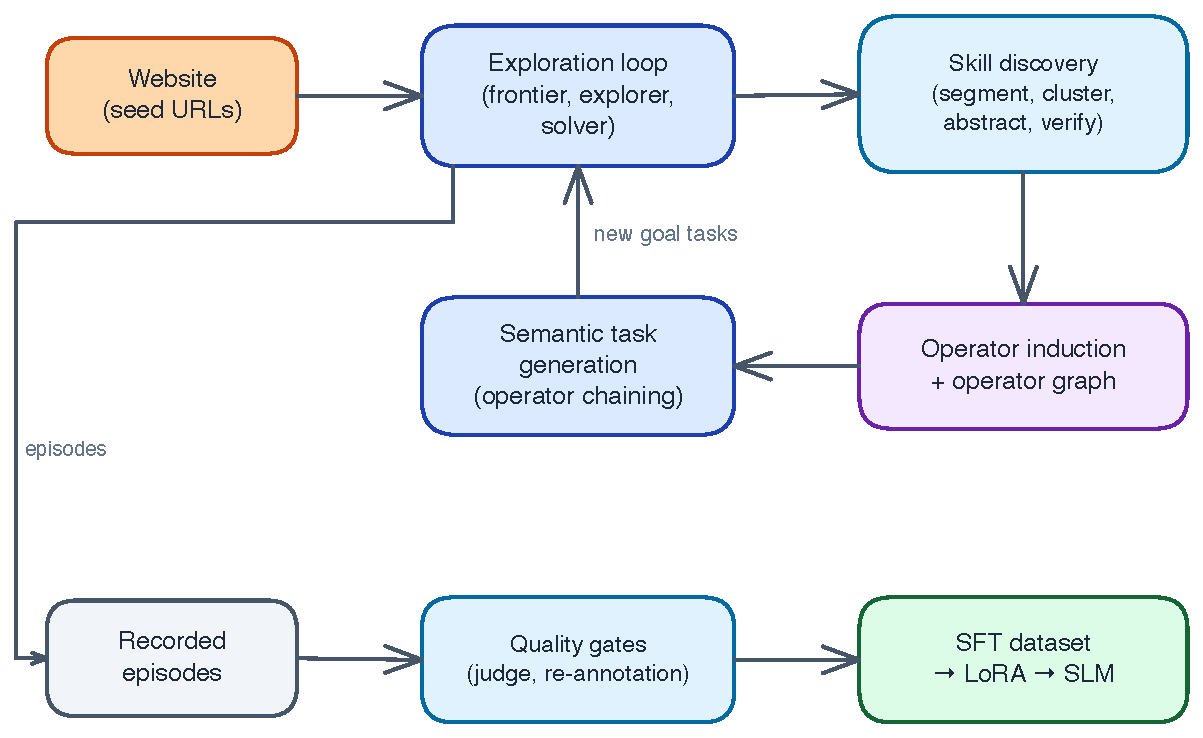
\includegraphics[width=\textwidth]{Figures/fig_pipeline.pdf}
\caption[Overview of the HSGE pipeline]{Overview of the HSGE pipeline. The
exploration loop solves LLM-proposed low-level tasks on frontier pages;
discovered skills are lifted into planning operators, whose chains are fed
back into the loop as semantic tasks. All recorded episodes pass through
quality gates before becoming fine-tuning data.}
\label{fig:pipeline}
\end{figure}

The pipeline operates as a loop. An \emph{explorer} proposes concrete,
page-grounded tasks on each visited page, and a \emph{solver} agent attempts
them in a real browser, producing interaction trajectories. A discovery
component segments these trajectories, clusters recurring segments, abstracts
each mature cluster into a reusable \emph{skill}, and lifts verified skills
into planning \emph{operators} with explicit preconditions and effects.
Chaining operators over the resulting graph yields composed, long-horizon
goal tasks --- the \emph{semantic tasks} --- which are fed back into the same
solver, closing the loop. Every attempted task, whether low-level or
semantic, is recorded as an episode; episodes then pass through automated
quality gates and are compiled into the SFT dataset used to fine-tune the
target SLM.

Three design principles run through the pipeline:

\begin{itemize}
  \item \textbf{P1 --- Verify before reuse.} Nothing is trusted on first
  sight. A skill is admitted only after it has recurred across independent
  trajectories; a declared task success is re-checked by an independent
  judge; an induced operator is rejected if its effects are vacuous.
  \item \textbf{P2 --- Graph over flat.} Instead of a flat pool of pages or
  memories, HSGE maintains a two-level graph (Section~\ref{sec:method-graph}).
  The low level records where the agent has been; the high level records what
  the agent can \emph{do}, and how those capabilities connect.
  \item \textbf{P3 --- A two-tier task hierarchy.} LLM-proposed
  \emph{low-level tasks} (Section~\ref{sec:method-exploration}) drive
  exploration and supply the raw material for skill discovery. \emph{Semantic
  tasks} (Section~\ref{sec:method-semantic}) are generated only from the
  operator graph, by composing verified capabilities into goals that no
  single page suggests.
\end{itemize}

\section{Two-Level Graph Representation}
\label{sec:method-graph}

\begin{figure}[htbp]
\centering
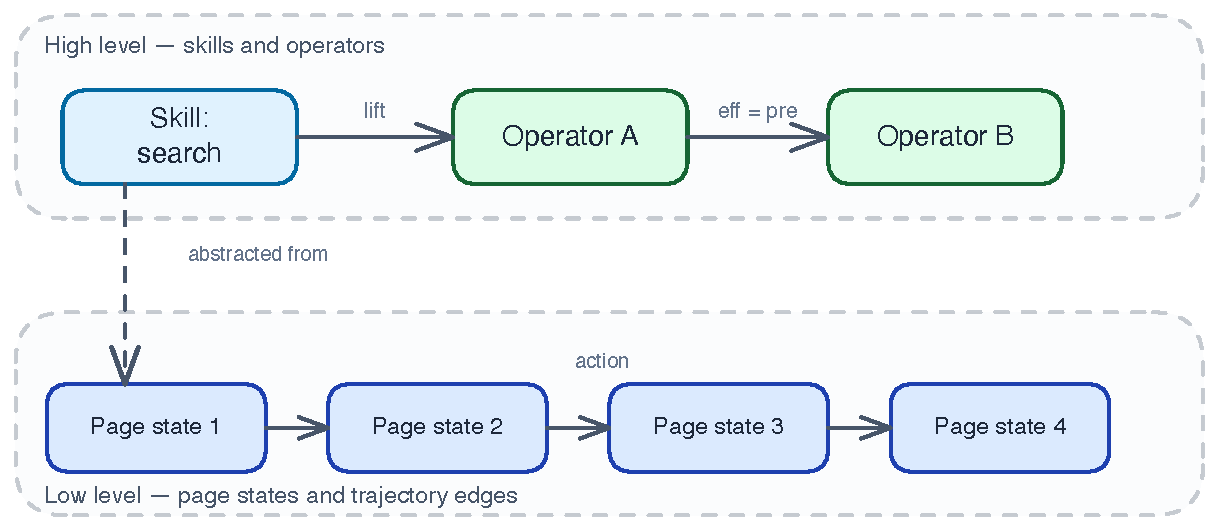
\includegraphics[width=0.95\textwidth]{Figures/fig_twolevel.pdf}
\caption[The two-level graph]{The two-level graph. The low level records
visited page states and the trajectory edges (actions) between them; the high
level records skills, lifted into planning operators and wired by composition
edges where one operator's effect matches the next one's precondition. Skills
are grounded in the low level through abstraction and initiation/effect
links.}
\label{fig:twolevel}
\end{figure}

\subsection{The website as a decision process}

We model the website as a partially observable decision process. At each step
the agent observes $o = (u, x)$, where $u$ is the current URL and $x$ is the
\emph{accessibility tree} (axtree) of the page: a text serialization of the
visible interface elements, each carrying a stable element identifier. The
agent acts through a fixed action space $\mathcal{A}$
(Table~\ref{tab:actions}), which covers element interaction, navigation, tab
management, and two terminal actions that end an episode: answering the user
and declaring the task infeasible. A \emph{trajectory} is the sequence
$\tau = \langle (o_0, a_0), (o_1, a_1), \dots \rangle$ produced while
attempting one task.

\begin{table}[H]
\centering
\caption[The solver's action space]{The solver's action space. Element
arguments refer to identifiers shown in the accessibility tree.}
\label{tab:actions}
\small
\begin{tabular}{L{5.4cm} L{7.8cm}}
\toprule
\textbf{Action} & \textbf{Meaning} \\
\midrule
\texttt{click(id)} & Click the element \texttt{id}. \\
\texttt{fill(id, text)} & Type \texttt{text} into the field \texttt{id}. \\
\texttt{select\_option(id, opt)} & Choose \texttt{opt} in the dropdown \texttt{id}. \\
\texttt{press(id, key)} & Send a keyboard shortcut to \texttt{id}. \\
\texttt{goto(url)}, \texttt{go\_back()} & Navigate directly / go back in history. \\
\texttt{new\_tab()}, \texttt{tab\_focus(i)}, \texttt{tab\_close()} & Tab management. \\
\texttt{send\_msg\_to\_user(text)} & Terminal: report the answer or completion. \\
\texttt{report\_infeasible(reason)} & Terminal: declare the task impossible. \\
\bottomrule
\end{tabular}
\end{table}

\subsection{Low level: page states and trajectory edges}

The low level of the graph records concrete experience: nodes are visited
page states, identified by URL and by a hash of the initial axtree, and edges
are the actions the agent actually executed between them. Hashing page
content, rather than trusting URLs alone, matters in practice: two distinct
URLs frequently render the same page, and revisiting them would waste an
entire exploration budget on content the agent has already seen.

\subsection{High level: skills as options}

A \emph{skill} is a reusable, parameterized capability, formalized in the
options framework~\cite{sutton1999options} as a triple
$\sigma = \langle I, \pi, \beta \rangle$: an initiation set $I$ (page states
where the skill applies), a policy $\pi$ (the action procedure), and a
termination condition $\beta$. Concretely, HSGE represents a skill as a
\emph{skill card}: a name, a natural-language description, a list of typed
parameter slots (for example a search query or a form value), and links to
the member trajectory segments it was abstracted from. Skill nodes are wired
to low-level states by initiation and effect edges, and to each other by
composition edges, forming the high-level graph.

\subsection{Operators: preconditions and effects}

Planning over raw skills is difficult because their applicability is
implicit. HSGE therefore lifts each verified skill into an
\emph{operator} in the classical STRIPS style~\cite{fikes1971strips}:
$\omega = \langle \mathit{pre}, \mathit{eff} \rangle$, where $\mathit{pre}$
and $\mathit{eff}$ are sets of natural-language predicates such as ``user is
viewing a project's issue list''. Unlike classical planning, the predicate
vocabulary is not fixed in advance: predicates are authored freely by an LLM
during induction and then \emph{canonicalized} into stable identifiers by an
embedding-based clusterer (Section~\ref{sec:method-semantic}), so that two
paraphrases of the same condition resolve to the same predicate. The
\emph{operator graph} draws an edge from operator $\omega_1$ to $\omega_2$
whenever an effect of $\omega_1$ satisfies a precondition of $\omega_2$;
paths in this graph are executable multi-skill plans.

\subsection{Task terminology}

Throughout this thesis we distinguish two tiers of tasks. A \emph{low-level
task} is a short, page-grounded instruction proposed by the explorer while
visiting a page (for example, ``open the most recently updated merge
request''). A \emph{semantic task} is a long-horizon goal generated from the
operator graph by chaining at least two operators; it exists only because the
graph exists, and it is the central product of the method.

\section{Graph-Guided Exploration}
\label{sec:method-exploration}

Exploration must answer three questions at every step: \emph{where} to go
next, \emph{what} to try there, and \emph{how} to try it. HSGE assigns these
to the frontier, the explorer, and the solver, respectively.

\subsection{Frontier management}
\label{sec:method-frontier}

The frontier is a priority queue over candidate URLs with two tiers of
candidates. \emph{Tier~0} contains URLs the agent actually reached while
solving tasks, together with pages left open in browser tabs; these are
admitted directly, subject only to allow/deny and visited checks, because
reaching them is itself evidence that they matter. \emph{Tier~1} contains
hyperlinks mined from each visited page's DOM. Mining hyperlinks is
essential: growth would otherwise depend entirely on task-driven navigation,
and a page whose tasks are all informational would contribute nothing to the
frontier --- a failure mode we return to in Chapter~\ref{ch:discussion}.

Mined links, however, arrive in bulk and are dominated by near-duplicates
(every post, comment, and user profile of a forum shares one page shape). To
keep them from flooding the queue, each URL is normalized into a
\emph{URL template}: the scheme, query, and fragment are dropped, and
identifier-like path segments --- together with everything after them --- are
replaced by wildcards, so that
\begin{center}
\texttt{/f/AskReddit/comments/12345/title}
$\;\rightarrow\;$
\texttt{/f/AskReddit/comments/*/*}.
\end{center}
At most $c$ pages per template are
visited (default $c = 3$), and the cap is re-checked lazily when a candidate
is popped, since a template's visit count grows during the run. Within
tier~1, candidates from unseen templates are preferred, then shallower pages,
then insertion order. Algorithm~\ref{alg:frontier} summarizes the loop; a
node whose initial page content hashes identically to an already-visited node
is skipped outright.

\begin{algorithm}[H]
\caption{Graph-guided exploration loop}
\label{alg:frontier}
\begin{algorithmic}[1]
\State $F \gets$ priority queue seeded with start URLs; $V \gets \emptyset$
\While{$F \neq \emptyset$ \textbf{and} node budget remains}
  \State $u \gets \textsc{Pop}(F)$ \Comment{key: (tier, template novelty, depth, seq)}
  \If{template cap of $u$ exhausted \textbf{or} $\textsc{Hash}(u) \in V$} \textbf{continue} \EndIf
  \State $V \gets V \cup \{\textsc{Hash}(u)\}$
  \State $T \gets \textsc{Explorer}(u)$ \Comment{low-level tasks, Sec.~\ref{sec:method-lowlevel}}
  \State $T \gets T \cup \textsc{SemanticTasks}()$ \Comment{operator chains, Sec.~\ref{sec:method-semantic}}
  \For{task $t \in T$}
    \State $\tau \gets \textsc{Solver}(u, t)$; record episode; $\textsc{Discovery}(\tau)$
    \State add URLs reached in $\tau$ to $F$ as tier~0
  \EndFor
  \State mine hyperlinks of $u$; add as tier~1 under template caps
\EndWhile
\end{algorithmic}
\end{algorithm}

\subsection{Low-level task proposal}
\label{sec:method-lowlevel}

On each frontier page, an LLM-based \emph{explorer} proposes up to $k$
concrete tasks (default $k = 6$) grounded in the page content. Each proposal
is returned in a structured form with an explicit type field ---
\texttt{INFO} (information seeking), \texttt{NAV} (navigation), or
\texttt{MOD} (state modification) --- rather than as free text with an
embedded tag, which production runs showed models do not reliably emit. The
classification is load-bearing: in a \emph{read-only} mode used on shared
sites, \texttt{MOD} tasks and any task the model failed to classify are
dropped fail-closed, since an unclassifiable task might be a modification in
disguise.

Two mechanisms keep proposals diverse. First, the explorer persists for the
whole run and remembers every task text it has already proposed; recent
proposals are echoed back into the prompt as negative context, and near
duplicates are additionally dropped in code. Without this, a large fraction
of proposals degenerate into sitewide navigation boilerplate repeated on
every page. Second, when the proposal list must be truncated to $k$,
information-seeking tasks are cut first: solving an \texttt{INFO} task never
navigates anywhere, so it can never grow the frontier.

These proposals are deliberately \emph{low-level}: each is scoped to what a
single page affords. Their role is to generate diverse, realistic
trajectories --- the raw material from which skills, and eventually semantic
tasks, are derived.

\subsection{The task solver}
\label{sec:method-solver}

\begin{figure}[htbp]
\centering
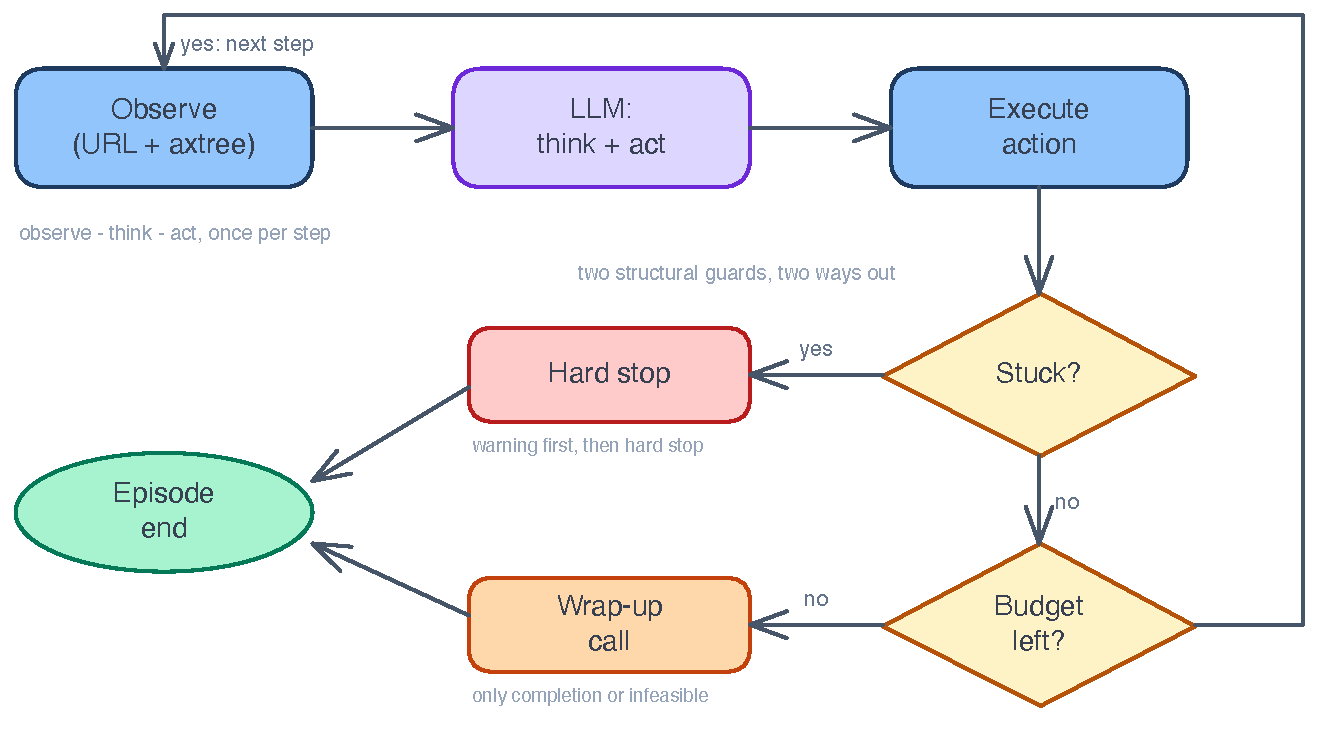
\includegraphics[width=\textwidth]{Figures/fig_solver.pdf}
\caption[The solver loop with structural guards]{The solver's
observe--think--act loop. A stuck-loop guard hard-stops the episode when
actions repeat on the same target with no observable change; an exhausted
step budget triggers a single wrap-up call that may only declare success or
infeasibility.}
\label{fig:solver}
\end{figure}

The \emph{solver} is a ReAct-style agent loop~\cite{yao2023react}: at each
step it receives the goal, the current URL, the (length-capped) accessibility
tree, and a window of its recent actions, each annotated with its observed
outcome (``now at $\langle$url$\rangle$'', ``page changed'', or ``no
change''), and it responds with a thought and one action from
Table~\ref{tab:actions}. If an action fails to execute, the error message is
fed back at the next step so the agent can recover instead of aborting.

Two structural guards bound the loop. First, the solver tracks whether each
action changed the observation and which target it acted on. A trailing run
of actions on the \emph{same target} with \emph{no observable change} first
triggers a warning injected into the prompt, and then --- because production
runs showed that a textual warning alone does not reliably stop a model from
re-clicking an inert element --- a hard stop that ends the episode. Requiring
``no observable change'', rather than merely a repeated action string,
prevents the guard from misfiring on legitimate multi-step sequences that
reuse one element across different pages. Second, when the step budget is
exhausted on a task without a programmatic goal check, the solver makes one
final text-only \emph{wrap-up} call that may only answer
\texttt{send\_msg\_to\_user} (declaring completion) or
\texttt{report\_infeasible}; anything else is discarded. Infeasibility is a
first-class outcome: it is never executed in the browser, never retried, and
never fed to skill discovery, but it \emph{is} kept as a training signal
(Section~\ref{sec:method-data}), teaching the model when to give up.

\section{Skill Discovery}
\label{sec:method-skills}

Every completed trajectory flows through a four-stage discovery pipeline:
segmentation, clustering, abstraction, and verification
(Figure~\ref{fig:discovery}).

\begin{figure}[htbp]
\centering
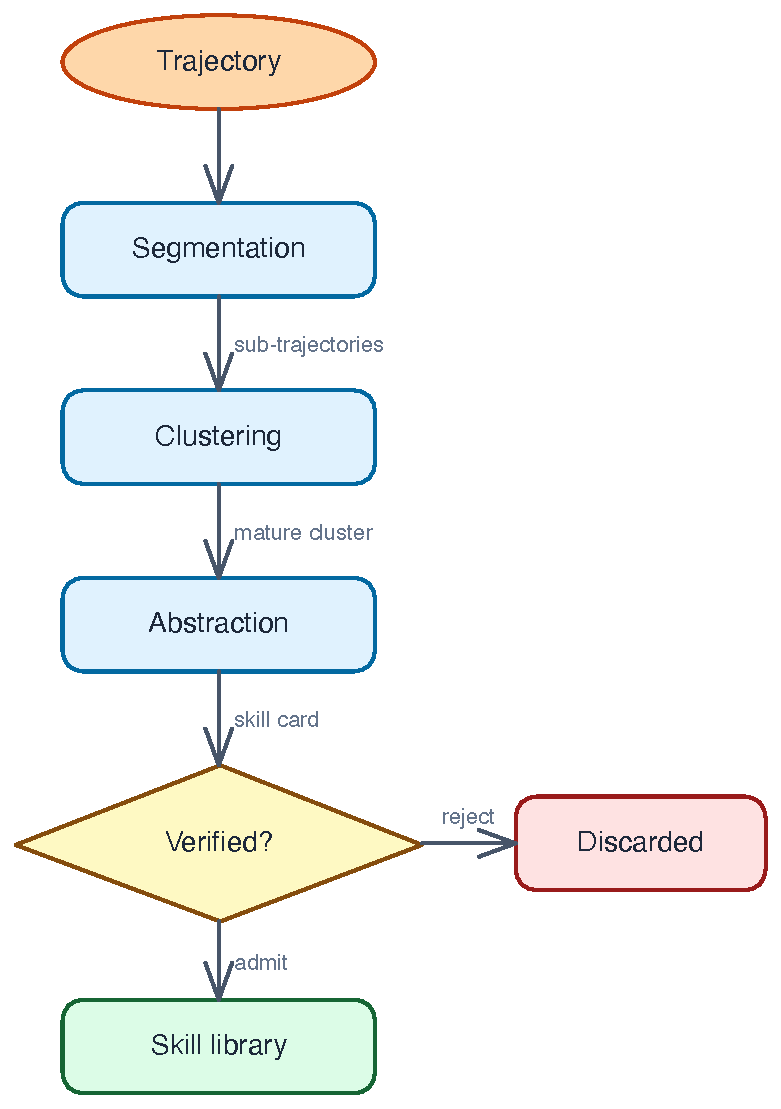
\includegraphics[width=0.48\textwidth]{Figures/fig_discovery.pdf}
\caption[The skill discovery pipeline]{The skill discovery pipeline. A
completed trajectory is segmented into sub-trajectories, streamed into
clusters, abstracted into a skill card, and admitted to the library only if
it passes verification; otherwise it is discarded.}
\label{fig:discovery}
\end{figure}

\subsection{Segmentation}

A trajectory typically interleaves several distinct behaviors (search, then
filter, then open a result). Segmentation cuts it into coherent
\emph{sub-trajectories}. Candidate cut points are seeded by two signals: URL
changes and drops in similarity between consecutive accessibility trees ---
the latter catches in-page transitions, such as a modal dialog opening, that
never touch the URL. An LLM then arbitrates the candidates, merging or
confirming cuts; its output is validated against the candidate set, and
trivial one-step navigation segments are merged into a neighbor.

\subsection{Streaming clustering}

Each sub-trajectory is embedded (using a sentence-encoder
representation~\cite{reimers2019sbert}) and assigned to a cluster by a
streaming, nonparametric clusterer in the DP-means
family~\cite{kulis2012dpmeans}: an incoming segment joins the nearest cluster
if its cosine similarity exceeds a threshold, and founds a new cluster
otherwise. The number of skills is therefore not fixed in advance, and
clustering happens online, during exploration, rather than in a separate
batch phase.

\subsection{Abstraction}

When a cluster matures --- it has recurred a configurable number of
independent times --- an LLM abstracts it into a \emph{skill card}: a name, a
description, and typed parameter slots that generalize over the concrete
values seen in the members (for example, the particular search string). The
member segments are retained as grounding evidence.

\subsection{Verification}

Following principle P1, a skill is admitted to the library only after
verification. In the deterministic mock environment used for development,
verification executes the skill in $k$ held-out contexts and requires every
run to succeed. On live websites, where re-execution is expensive and has
side effects, admission instead relies on recurrence across independent
trajectories (the maturity threshold) combined with outcome checks on the
episodes involved; Chapter~\ref{ch:discussion} discusses this trade-off.

\section{Semantic Task Generation via Operator Chaining}
\label{sec:method-semantic}

This section describes the centerpiece of the method: how the graph turns
verified skills into new, long-horizon training tasks that no single page
proposal would produce (Figure~\ref{fig:semantic}).

\begin{figure}[htbp]
\centering
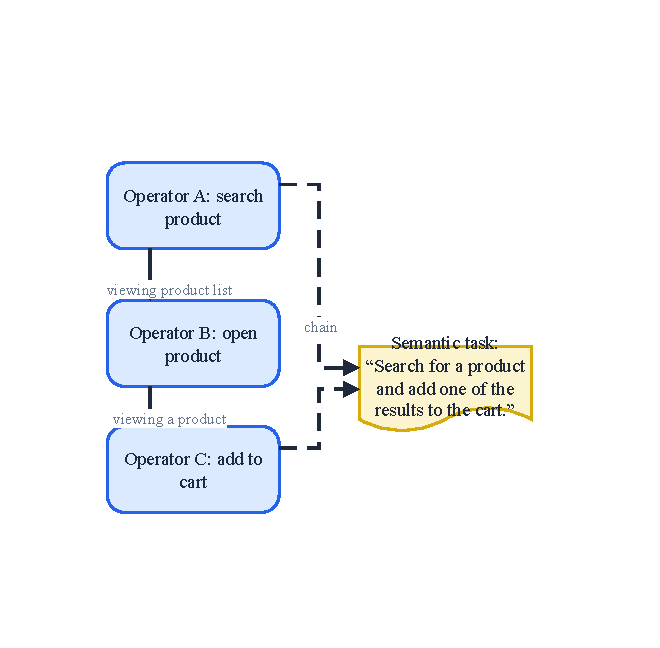
\includegraphics[width=0.78\textwidth]{Figures/fig_semantic.pdf}
\caption[Semantic task generation via operator chaining]{Semantic task
generation by operator chaining. Each edge is labelled with the shared state
where one operator's effect matches the next operator's precondition; chaining
the operators yields a single long-horizon semantic task that no individual
page proposes.}
\label{fig:semantic}
\end{figure}

\subsection{Operator induction}

When a skill is admitted, an LLM \emph{inducer} examines its skill card
together with the boundary observations (the pages before and after) of a few
member segments, and authors the skill's preconditions and effects as
natural-language predicates. Free-form authoring alone, however, fragments
the vocabulary: measured on a production run, embedding similarity failed to
unify a true paraphrase pair (scoring 0.570, below the merge threshold of
0.6) while scoring a false pair higher (0.606). Induction is therefore
\emph{vocabulary-aware}: the prompt includes the registry's existing
predicate labels --- the most frequent and most recent entries --- with an
instruction to reuse an equivalent predicate's exact text verbatim rather
than rephrase it.

Induced operators pass through an \emph{anti-tautology gate}. Any effect that
merely restates a precondition is dropped ($\mathit{eff} \leftarrow
\mathit{eff} \setminus \mathit{pre}$); a skill left with no novel effect is
rejected outright rather than promoted. This gate exists because, without it,
a majority of induced operators in early runs encoded no state change at all
--- and an operator that changes nothing can never chain toward anything new.
An operator is marked \emph{terminal} if one of its member episodes actually
reached a configured goal state, or if the inducer flags it as
goal-completing.

\subsection{Predicate canonicalization}

Each authored predicate is resolved against a \emph{predicate registry},
which reuses the same cosine-threshold clustering as the skill library but
with merging disabled, so identifiers stay stable once assigned: a new
predicate either joins an existing canonical cluster (and adopts its
identifier) or founds a new one. Operators thus share a common, growing
vocabulary $P = \{p_0, p_1, \dots\}$, and the planner can match effects to
preconditions by identifier equality --- keeping classical set-based planning
intact over an open, LLM-authored vocabulary.

\subsection{Chaining operators into semantic tasks}

The operator graph connects $\omega_1 \rightarrow \omega_2$ whenever an
effect of $\omega_1$ canonically matches a precondition of $\omega_2$. A
bounded depth-first enumeration lists all simple chains of length at least
two (with circuit breakers on path length and path count, since simple-path
enumeration is combinatorial in dense graphs). Each distinct chain becomes
one composed \emph{goal task}: its instruction is generated from the chained
skills' descriptions, and its starting point is the initiation URL recorded
for the first operator. For example, if exploration separately discovered
``search the product catalog'' and ``add a listed product to the cart'', the
chain of the two yields a task of the form \emph{``search for a product and
add one of the results to the cart''} --- a goal grounded in verified
capabilities, but never proposed by any single page.

Semantic tasks are scheduled conservatively: each distinct chain is attempted
once per run, and at most a fixed number of new chains is attempted per
visited node. Verification is deterministic when it can be: if the chain's
last operator is terminal and the site has a configured terminal predicate
(such as an order-confirmation URL), success is checked programmatically.
Otherwise the episode is self-graded through the solver's terminal answer and
then re-checked offline by the judge (Section~\ref{sec:method-data}). When
the graph is still too shallow to chain --- fewer than two connected
operators --- the system falls back to planning directly toward the terminal
predicate where one exists, so goal-directed data collection begins before
the graph has matured.

Semantic tasks matter for the end goal --- training data --- in two ways.
They extend the \emph{length distribution} of collected trajectories beyond
what single-page tasks produce, and they carry compositional structure: the
episode demonstrably strings multiple verified capabilities together, which
is precisely the behavior a small model most needs demonstrations of.

\section{Data Curation}
\label{sec:method-data}

Raw episodes are not yet training data. Three offline stages turn them into a
dataset while enforcing principle P1 end to end (Figure~\ref{fig:curation}).

\begin{figure}[htbp]
\centering
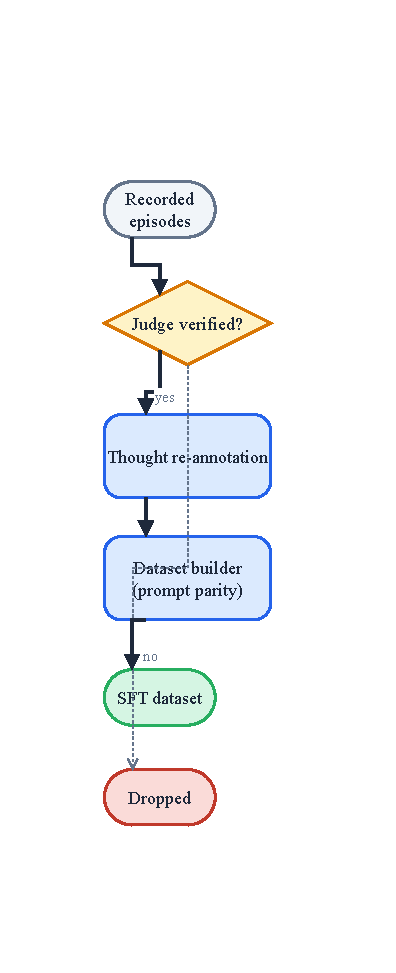
\includegraphics[width=0.50\textwidth]{Figures/fig_curation.pdf}
\caption[The data curation pipeline]{The data curation pipeline. Recorded
episodes are re-checked by an independent judge, their thoughts re-annotated,
and compiled by a prompt-parity dataset builder; declared successes that fail
judging are dropped.}
\label{fig:curation}
\end{figure}

\subsection{Independent judging of declared successes}

A solver that answers ``done'' has, in effect, graded its own homework. A
\emph{judge} pass re-examines every declared-success episode with a stronger
LLM, comparing the goal against the episode's own final state (URL and page
content), and records a verdict alongside the original outcome. The verdict
is additive --- original outcomes are never overwritten --- and the dataset
builder can be instructed to keep only judge-verified successes, dropping
never-judged episodes rather than silently trusting them.

\subsection{Thought re-annotation}

The solver's spontaneous thoughts are uneven in quality, and they are the
imitation target for the fine-tuned model. A re-annotation pass rewrites each
step's thought into a structured form composed of: a terse assessment of the
current state; a reflection when the previous action made no progress; the
step's current \emph{subgoal}, recovered by replaying the same segmentation
used during discovery over the recorded trajectory; and, only on a task's
final step, an explicit completion check against the goal. Crucially, the
subgoal appears only in the assistant \emph{target}, never in the user
prompt: at inference time no component exists to supply ``the current
subgoal'' as an input, and training must not assume one.

\subsection{Dataset construction with prompt parity}

The final builder compiles episodes into instruction-tuning examples under a
strict \emph{prompt parity} rule: the training-time prompt is byte-identical
in structure to the live solver's. The system prompt is imported from the
solver rather than duplicated; the page observation is capped by the same
truncation routine with the same explicit truncation marker; and history
lines are rendered with the same outcome annotations the live agent sees.
Steps whose recorded action failed to execute are excluded both as targets
and from later steps' history --- the error, after all, was never part of the
live agent's own history either. Episodes that ended in a justified
\texttt{report\_infeasible} are kept as valid targets. Each example carries
its trajectory identifier and step index, enabling trajectory-aware batching,
and examples are ordered easy-to-hard (shorter, verified episodes first) to
form a curriculum.

\section{Fine-Tuning the Small Language Model}
\label{sec:method-sft}

The target model is Qwen3.5-9B~\cite{yang2025qwen3}, fine-tuned with
LoRA~\cite{hu2022lora} using the LLaMA-Factory
framework~\cite{zheng2024llamafactory}. Two details are load-bearing. First,
the train/validation split is performed \emph{by trajectory}, never by step:
steps of one episode are strongly correlated, and splitting them across sets
would leak information. Second, the model family emits explicit reasoning
segments by default, while our targets are bare thought--action pairs; the
chat template must therefore disable the model's built-in ``thinking'' mode
consistently at training \emph{and} inference time. After training, the
adapter is merged and the model is served with vLLM~\cite{kwon2023vllm},
again with thinking disabled on every request, so the deployed model sees
exactly the distribution it was trained on --- the serving-side counterpart
of prompt parity.

\section{Implementation Notes}
\label{sec:method-impl}

HSGE is implemented in Python. Table~\ref{tab:modules} maps the pipeline
stages to modules. Two implementation decisions deserve mention. First, every
LLM-backed role --- explorer, solver, segmenter, abstractor, verifier,
inducer, judge, re-annotator --- is independently configurable, so cheap
models can serve high-volume roles while stronger models are reserved for
induction and judging. Second, the entire pipeline runs against deterministic
mock backends (a scripted LLM, a hash-based embedder, and a simulated
website) with no code changes: real backends are subclass swaps. This seam
makes the discovery logic unit-testable with exact assertions, and it
decouples algorithm development from API cost and website availability.
Artifacts (skills, operators, the graph, per-node results, and an event log)
are persisted after every explored node, so an interrupted run still leaves a
consistent snapshot.

\begin{table}[H]
\centering
\caption[Pipeline stages and implementation modules]{Pipeline stages and the
modules implementing them.}
\label{tab:modules}
\begin{tabular}{L{5.2cm} L{8.0cm}}
\toprule
\textbf{Stage} & \textbf{Module(s)} \\
\midrule
Exploration loop, frontier & \texttt{webarena/runtime}, \texttt{webarena/browser} \\
Task proposal and solving & \texttt{webarena/agents} \\
Segmentation & \texttt{segmentation}, \texttt{discovery} \\
Clustering, skill library & \texttt{clustering}, \texttt{abstraction}, \texttt{library} \\
Operators and planning & \texttt{operators}, \texttt{operator\_induction}, \texttt{predicate\_registry} \\
Data curation & \texttt{judge\_episodes}, \texttt{reannotate\_thoughts}, \texttt{build\_sft\_dataset} \\
Training and serving & LLaMA-Factory configs, vLLM scripts \\
\bottomrule
\end{tabular}
\end{table}

\vspace{1em}
\noindent
With the method in place, the next chapter turns to its empirical evaluation:
how much data the pipeline collects in practice, and whether fine-tuning on
that data improves a small model on the official WebArena benchmark.


\chapter{Experiments}
\label{ch:experiments}

This chapter (1) describes the experimental environment and evaluation
protocol, (2) reports data-collection results, (3) reports fine-tuning
results, (4) presents the main evaluation on the official WebArena task
suites of four sites, and (5) analyzes the results.

% NOTE: this chapter is scaffolded first and will grow as the remaining
% experiments finish (see [TO ADD] markers). Current numbers come from the
% GitLab evaluation of 2026-07-15.

\section{Experimental Setup}
\label{sec:exp-setup}
% TODO: self-hosted WebArena instances; vast.ai A100-80GB for training and
% serving; per-role LLM configuration table (from config.yaml); run
% parameters; evaluation via BrowserGym scored environments + official
% evaluators, replaying the terminal answer action.
\textit{[To be written — see outline 07, section 4.1.]}

\section{Data Collection Results}
\label{sec:exp-data}
% TODO: per-run statistics (nodes, tasks proposed/solved/infeasible, skills,
% operators, chains); final dataset: 370 examples (352 train / 18 val);
% 1-2 representative examples of a discovered skill and a semantic task.
\textit{[To be written — see outline 07, section 4.2.]}

\section{Fine-Tuning Results}
\label{sec:exp-sft}
% TODO: LoRA training curves (train loss 0.32 / eval loss 0.24), time and
% cost table (docs/14).
\textit{[To be written — see outline 07, section 4.3.]}

\section{Main Evaluation on WebArena}
\label{sec:exp-main}
% Evaluation on FOUR sites: Shopping, Shopping Admin, GitLab, Reddit.
% Current: GitLab — base 10/180 (5.56%) vs fine-tuned 12/180 (6.67%).
% Present as a directional signal (n=1 per task) until repeats (Sec. 4.5).
% [TO ADD] Shopping / Shopping Admin / Reddit results + per-site table.
\textit{[To be written — see outline 07, section 4.4.]}

\section{Statistical Repeats}
\label{sec:exp-stats}
% [TO ADD] >=3-5 repeated runs (or seeds) per model -> mean +/- SD, 95% CI,
% non-parametric significance test. Priority #1.
\textit{[Planned — see outline 07, section 4.5.]}

\section{Ablation Studies}
\label{sec:exp-ablation}
% [TO ADD] (a) graph-explore data vs flat-explore data at equal budget;
% (b) with/without judge pass; (c) with/without thought re-annotation;
% (d) cross-site analysis from the 4-site results.
\textit{[Planned — see outline 07, section 4.6.]}

\section{Analysis}
\label{sec:exp-analysis}
% TODO: per-task-type breakdown, qualitative success/failure examples,
% failure taxonomy (feeds Chapter 5).
\textit{[To be written — see outline 07, section 4.7.]}


\chapter{Discussion}
\label{ch:discussion}

This chapter (1) interprets the experimental results of
Chapter~\ref{ch:experiments}, then distills the engineering experience gained
while building and operating the pipeline into lessons on (2) exploring live
websites, (3) guarding LLM agents structurally rather than through prompt
wording, (4) inducing high-quality planning operators, and (5) training and
serving small language models, before (6) summarizing these lessons as best
practices and (7) discussing threats to validity. Each lesson follows the
same pattern: a problem actually encountered in our runs, its diagnosis, the
fix, and the general principle we draw from it. Full incident details are
collected in Appendix~\ref{app:runs}.

\section{Interpreting the Results}
\label{sec:disc-results}

% TODO: refresh this section once the remaining three sites and the
% statistical repeats (Sections 4.5-4.6) are in.

The headline number so far --- an improvement from 5.56\% to 6.67\% task
success on the official GitLab suite --- deserves a careful reading rather
than a triumphant one. In absolute terms the gain is small, and with one
attempt per task it must be treated as a directional signal until the
repeated runs of Section~\ref{sec:exp-stats} are complete. What makes the
signal interesting is its cost profile: it was obtained from only 352
training examples, collected autonomously from a website with no human
annotation, and the fine-tuning itself took under half an hour on a single
GPU. The pipeline, in other words, moved a small model in the right direction
with a remarkably small amount of data; the open question is how far the
trend continues as data collection scales, which the cross-site results of
Section~\ref{sec:exp-main} will begin to answer.

Three factors plausibly bound the current gain. First, dataset size: 352
examples is two to three orders of magnitude below typical agent fine-tuning
corpora, so the model sees each interaction pattern only a handful of times.
Second, coverage: the training data was collected on a subset of site areas,
while the benchmark draws tasks from the whole site. Third, the base model
itself: a 9B-parameter model fine-tuned with supervised trajectories alone
cannot be expected to recover capabilities --- long-horizon planning,
self-correction --- that the trajectories only sparsely demonstrate. None of
these factors indicts the pipeline design; all three point to data volume
and breadth as the binding constraint, which is precisely the constraint the
pipeline is built to relax.

Equally important is what the end-to-end run \emph{demonstrated}: every stage
--- exploration, discovery, operator chaining, curation, training, serving,
and official evaluation --- executed against a real website without manual
intervention, and the quality gates rejected data that would otherwise have
polluted training (Section~\ref{sec:disc-slm}). The remainder of this chapter
reports what it took to make that sentence true.

\section{Lessons from Exploring Live Websites}
\label{sec:disc-exploration}

\subsection{Frontier starvation}

\textbf{Problem.} An early exploration run on the Reddit-style site stalled
at 57 of a budgeted 500 nodes: the frontier simply ran dry.
\textbf{Diagnosis.} The frontier then grew only from URLs the solver happened
to navigate to. Pages whose proposed tasks were all informational produced no
navigation at all, so entire regions of the site were never queued ---
exploration was hostage to which tasks the explorer happened to propose.
\textbf{Fix.} Hyperlink mining was added as a second frontier tier, with URL
templating and per-template caps to keep near-duplicate pages from flooding
the queue (Section~\ref{sec:method-frontier}).
\textbf{Lesson.} On a real website, \emph{reachability must not depend on
task-driven behavior}. Structural signals (links) and behavioral signals
(navigation) are complementary frontier sources, and the structural one needs
explicit diversity controls because it arrives in bulk.

\subsection{Task proposal collapse}

\textbf{Problem.} In one production run, 46\% of all proposed tasks were
near-identical across pages --- variations of ``go to the Forums page''
re-proposed on nearly every node.
\textbf{Diagnosis.} Every page of a site shares its global navigation menu,
and an explorer prompted page-by-page has no memory of what it already
proposed elsewhere.
\textbf{Fix.} The explorer now persists for the whole run: recent proposals
are echoed into its prompt as negative context, and near-duplicates are
additionally dropped in code (Section~\ref{sec:method-lowlevel}).
\textbf{Lesson.} Diversity of generated tasks is a \emph{run-level} property,
not a page-level one; it must be enforced by state that outlives any single
LLM call.

\subsection{Unreliable pages}

\textbf{Problem.} A single slow page --- a navigation timeout on one mined
URL --- crashed an entire multi-hour exploration run.
\textbf{Diagnosis.} Browser operations were implicitly trusted; one
unhandled exception anywhere in node processing propagated to the top level.
\textbf{Fix.} Every browser operation is now fail-soft: a node that cannot be
opened is logged, recorded with its error, and skipped, while genuinely
unexpected exceptions still abort the run loudly. Artifacts are persisted
after every node, so even an aborted run leaves a consistent, resumable
snapshot.
\textbf{Lesson.} Treat every interaction with a live website as an
operation that \emph{will} eventually fail, and decide per operation whether
failure is survivable; make the run's progress durable at the finest
granularity the budget allows.

\subsection{Shared, mutable state}

\textbf{Problem.} Benchmark websites are shared and stateful: a careless
agent can pollute --- or destroy --- the environment other runs depend on.
\textbf{Fix.} Three layers of discipline: a read-only mode that drops
state-modifying tasks fail-closed (any task the explorer fails to classify is
treated as modifying); a standing rule forbidding account-level destructive
tasks regardless of mode; and, for evaluation on a live shared instance, an
intent-based classification of benchmark tasks into read-only and
write-mutating subsets so that two machines can sweep the same site
concurrently without interfering (Section~\ref{sec:disc-slm}).
\textbf{Lesson.} On shared infrastructure, safety must be
\emph{fail-closed}: the burden of proof lies on a task being harmless, not on
it being harmful.

\section{Structural Guardrails over Prompt Nudges}
\label{sec:disc-guardrails}

A recurring theme of our runs is that instructing a model to behave is not
the same as making the system behave. The incidents below each began as a
prompt-level convention that a real model quietly violated, and each ended as
a structural mechanism that does not depend on model obedience.

\subsection{Tag conventions do not survive contact with real models}

\textbf{Problem.} Task proposals were originally classified by a leading
\texttt{[INFO]}/\texttt{[NAV]}/\texttt{[MOD]} tag that the explorer was
instructed to emit. In a real run, 89\% of proposals carried no tag at all.
\textbf{Diagnosis.} The model's natural tendency was to return the
classification as a structured \texttt{type} field --- which the parser
discarded --- rather than as a bracket inside a string. Worse, the safety
check for modifying tasks was a literal substring test on \texttt{[MOD]}, so
an untagged destructive task would have sailed through it.
\textbf{Fix.} Proposals are now requested and parsed as structured objects
with an explicit type field; anything unclassifiable is tagged
\texttt{UNKNOWN} and dropped in read-only mode.
\textbf{Lesson.} Ask models for \emph{structure}, not for formatting
conventions inside free text --- and never build a safety check on a
convention the model may not follow.

\subsection{The stuck loop, in two iterations}

\textbf{Problem.} Solvers wasted entire step budgets repeating an action that
visibly did nothing --- in one recorded episode, clicking the same inert
element for all fifteen steps.
\textbf{Diagnosis and first fix.} We added a warning, injected into the
prompt after two consecutive no-effect actions on the same target. The next
real run falsified the fix: the model kept clicking with the warning present
from the third call onward. It also revealed a subtlety --- the model
sometimes retried a stuck dropdown with different-looking but equally wrong
arguments, so matching identical action strings would miss the loop entirely.
\textbf{Second fix.} The loop detector now keys on the \emph{target} acted
on and on whether the observation changed; after a bounded number of
no-progress repeats, the episode is terminated outright, spending no further
LLM calls. Requiring ``no observable change'' keeps the guard from misfiring
on legitimate sequences that reuse one element across changing pages.
\textbf{Lesson.} A prompt warning is a suggestion; a budget is a mechanism.
When a model demonstrably ignores the suggestion, escalate to a mechanism ---
and validate the escalation on real behavior, not on the behavior the prompt
requests.

\subsection{Smaller incidents, same shape}

Three further incidents followed the same pattern and received the same style
of fix. Explorer-proposed information tasks sometimes contained their own
answers (``find the post titled X''), which a solver can ``solve'' without
learning anything; generation now instructs against it and leaky tasks are
filtered. Vision-attached calls occasionally returned empty responses
(upstream refusals); the agent retries once in text-only mode rather than
failing the step. And episodes that exhausted their budget originally ended
in an uninformative failure; they now receive one final text-only wrap-up
call whose \emph{only} admissible outputs are a completion claim or an
infeasibility report --- turning a silent timeout into a labeled outcome that
the dataset can use.

\section{Lessons from Operator Induction}
\label{sec:disc-operators}

The semantic-task mechanism of Section~\ref{sec:method-semantic} is only as
good as the operators it chains. Two failure modes surfaced when we audited
the operators induced in an early production run, and both led to structural
gates rather than prompt adjustments.

\subsection{Tautological operators}

\textbf{Problem.} Three of the four operators induced in that run had effect
sets identical to their precondition sets.
\textbf{Diagnosis.} Asked to describe a skill's preconditions and effects,
an LLM finds it easiest to restate the context --- ``user is on the issue
list'' before, ``user is on the issue list'' after. Such an operator encodes
no state change, so it can never appear mid-chain and never lead anywhere
new; left unchecked, tautologies would have filled the operator graph with
dead nodes.
\textbf{Fix.} The anti-tautology gate: effects that restate a precondition
are dropped, and a skill left without novel effects is rejected from
promotion altogether, with the rejection logged.
\textbf{Lesson.} For LLM-authored symbolic artifacts, \emph{define validity
set-theoretically and enforce it in code}; do not rely on the prompt to
forbid degenerate answers.

\subsection{Synonymous predicates that embeddings cannot unify}

\textbf{Problem.} Chaining requires an effect of one operator to match a
precondition of another, but independently induced operators phrase the same
condition differently.
\textbf{Diagnosis.} We measured the embedding similarity of predicate pairs
from the same run: a true paraphrase pair scored 0.570 --- \emph{below} the
0.6 canonicalization threshold --- while a semantically different pair scored
0.606, above it. No threshold separates these cases; purely geometric
canonicalization cannot recover a shared vocabulary after the fact.
\textbf{Fix.} Prevention rather than cure: induction is vocabulary-aware.
The prompt presents the registry's existing predicate labels with an
instruction to reuse an equivalent one verbatim, so unification happens at
authoring time, where the model has full context, instead of at embedding
time, where only the surface strings remain.
\textbf{Lesson.} When two LLM outputs must later \emph{match}, share the
vocabulary at generation time; do not defer semantic unification to a
similarity metric.

\section{Pitfalls in Training and Serving SLMs}
\label{sec:disc-slm}

\subsection{The chat template is part of the model}

The target model family emits explicit reasoning segments by default, while
our training targets are bare thought--action pairs. The correct,
thinking-disabled chat template had to be identified from the training
framework's template registry rather than guessed from documentation, and the
same setting had to be applied again, per request, at serving time. A
mismatch on either side silently trains or evaluates a different
distribution than intended. The general point: \emph{template and decoding
configuration are part of the model artifact}, and train-time and
serve-time configurations must be pinned together.

\subsection{The prompt-fidelity bug}

The most instructive failure of the training phase produced no error at all.
A quick post-training smoke test, written with an \emph{approximation} of the
solver prompt, made the fine-tuned model emit natural-language descriptions
instead of executable actions --- which looked exactly like a failed
fine-tune. The model was fine; the test prompt was unfaithful. Re-testing
with the production prompt --- imported from the solver, not re-typed ---
produced correct actions. This incident is why prompt parity
(Section~\ref{sec:method-data}) is enforced by \emph{importing} the live
system prompt and its helper routines into the dataset builder and the
evaluation harness, never by duplicating them. Any test of a fine-tuned
agent is only as valid as the fidelity of its prompt to production.

\subsection{Dependency isolation}

Supporting a newly released model architecture required the development
version of the modeling library, which conflicted with the serving engine's
pinned requirements. Three isolated environments --- training, serving, and
evaluation --- resolved what no single environment could satisfy. Mundane,
but it converts an unsolvable version conflict into a routine setup step.

\subsection{Agents grade their own homework}

The judge pass exists because declared success is not success: a solver that
answers ``done'' has evaluated itself. Re-checking declared successes against
the episode's own final state caught self-graded failures before they became
training examples --- and the dataset builder's strict mode inverts the
default, dropping any declared success that was never judged rather than
trusting it. Under principle P1, \emph{unverified data is not neutral; it is
a liability that compounds through training}.

\subsection{Evaluating safely on shared live sites}

Running baseline and fine-tuned sweeps against one live site instance would
normally serialize a full working day of evaluation. Classifying benchmark
tasks by intent into read-only and write-mutating subsets let a second
machine evaluate the read-only subset concurrently with the first machine's
unrestricted sweep. The classification itself held two traps worth recording:
noun-phrase collisions (``merge request'' contains a verb only
syntactically; ``report bugs'' does not name the reporting action the regex
expected) and word insertion defeating naive phrase patterns (``open a
\emph{new} issue''). Transfer cost also mattered: moving the 1.7\,GB LoRA
adapter and re-merging locally beat moving an 18\,GB merged checkpoint.

\section{Best Practices}
\label{sec:disc-practices}

Table~\ref{tab:practices} condenses the lessons of this chapter into
practices we would adopt from the first day of a similar project.

\begin{table}[H]
\centering
\caption[Distilled best practices]{Distilled best practices for
LLM-agent data-collection pipelines on live websites.}
\label{tab:practices}
\small
\begin{tabular}{L{4.4cm} L{8.8cm}}
\toprule
\textbf{Practice} & \textbf{Rationale (section)} \\
\midrule
Verify, then admit & Skills, operators, and successes are liabilities until independently checked (\ref{sec:disc-slm}, \ref{sec:disc-operators}). \\
Prompt parity by import & Training data, live agent, and eval harness share one prompt source; duplication drifts (\ref{sec:disc-slm}). \\
Structure over conventions & Request typed fields from models; never parse safety-relevant information out of free text (\ref{sec:disc-guardrails}). \\
Mechanisms over warnings & Convert repeated model misbehavior into budgets and hard stops, validated on real runs (\ref{sec:disc-guardrails}). \\
Fail-soft browsing & Any page operation may fail; skip and log locally, crash only on the truly unexpected (\ref{sec:disc-exploration}). \\
Persist per node & Interrupted runs should leave consistent, resumable artifacts (\ref{sec:disc-exploration}). \\
Fail-closed safety & Unclassifiable tasks count as destructive; destructive account actions are banned outright (\ref{sec:disc-exploration}). \\
Share vocabulary at authoring time & Symbolic artifacts that must match later should be generated against a shared label set (\ref{sec:disc-operators}). \\
Pin template with model & Chat template and decoding flags are part of the artifact, for training and serving alike (\ref{sec:disc-slm}). \\
Log everything as events & A per-run event log makes post-hoc failure analysis --- most of this chapter --- possible at all (\ref{sec:disc-exploration}). \\
\bottomrule
\end{tabular}
\end{table}

\section{Threats to Validity}
\label{sec:disc-validity}

\textbf{Internal validity.} The evaluation to date runs each benchmark task
once per model; individual task outcomes on a live site are noisy, so the
measured gap could shift under repetition. The planned repeated runs
(Section~\ref{sec:exp-stats}) address this directly. Several quality gates
(the judge, the re-annotator) are themselves LLMs and inherit LLM biases;
we mitigate but do not eliminate this by checking judgments against concrete
final states rather than against transcripts alone.

\textbf{External validity.} All data and evaluation come from self-hosted
WebArena sites --- realistic, but four sites of one benchmark family ---
and from one 9B model. Claims are correspondingly scoped: we report that the
pipeline improves \emph{this} model on \emph{these} sites, and treat broader
generalization as future work rather than as an implication.

\textbf{Construct validity.} Task success against official evaluators is the
field-standard construct, but it is binary and end-state-based: it does not
credit partial progress, and semantic-task episodes verified by self-report
plus offline judging are a weaker construct than programmatically checked
ones. We keep the two verification regimes distinguishable in the data so
that stricter analyses remain possible.

\vspace{1em}
\noindent
These lessons, and the results they contextualize, complete the empirical
story of the thesis. The final chapter summarizes what was built and learned,
and where the work goes next.


\chapter{Conclusion}
\label{ch:conclusion}

This chapter (1) summarizes the products and contributions of the thesis,
(2) compares the achieved results against the initial objectives, and
(3) outlines directions for future work.

\section{Summary of Contributions and Products}
\label{sec:conc-summary}
% TODO: (1) the HSGE pipeline (source code, mock + real backends);
% (2) the semantic-task + trajectory SFT dataset; (3) the fine-tuned
% Qwen3.5-9B model; (4) official benchmark results on four WebArena sites;
% (5) the engineering experience report and reproduction tutorial.
% Restate the main message. Focus on strengths.
\textit{[To be written — see outline 07, section 6.1.]}

\section{Objectives versus Achievements}
\label{sec:conc-objectives}
% TODO: table mapping each objective from Section 1.4 to what was achieved.
\textit{[To be written — see outline 07, section 6.2.]}

\section{Future Directions}
\label{sec:conc-future}
% TODO: data scaling across sites (transfer machinery exists); RL/DPO on
% verified trajectories; smaller models (<=3B); online skill retrieval at
% inference time; broader benchmarks.
\textit{[To be written — see outline 07, section 6.3.]}


% Bibliography
\addcontentsline{toc}{chapter}{References}
\printbibliography[title={References}]

% Appendices
\appendix
\chapter{Detailed Design}
\label{app:design}

This appendix records the implementation detail that Chapter~\ref{ch:method}
deliberately omits: the module map, the data schema every stage exchanges,
the backend abstraction that lets the same pipeline run on mocks or on a live
browser, and the exact configuration used for the runs reported in
Chapter~\ref{ch:experiments}.

\section{Module map}
\label{app:design-modules}

Table~\ref{tab:app-modules} lists every module of the implementation with its
responsibility. The pipeline core is deliberately small: the whole discovery
path from a raw trajectory to an admitted skill is under 700 lines, which is
what makes the deterministic mock tests practical.

{\footnotesize
\begin{longtable}{@{}L{4.3cm}rL{8.0cm}@{}}
\caption[Module map of the HSGE implementation]{Module map. Line counts are of
the implementation only, excluding tests.}
\label{tab:app-modules}\\
\toprule
\textbf{Module} & \textbf{Lines} & \textbf{Responsibility} \\
\midrule
\endfirsthead
\toprule
\textbf{Module} & \textbf{Lines} & \textbf{Responsibility} \\
\midrule
\endhead
\bottomrule
\endfoot
\multicolumn{3}{@{}l}{\emph{Pipeline core (\texttt{hsge/})}} \\
\midrule
\texttt{schema.py}      & 129 & Shared data types: \texttt{Step},
\texttt{SubTrajectory}, \texttt{SkillCard}, \texttt{ParamSlot}, \texttt{Task} \\
\texttt{segmentation.py} & 138 & Candidate cuts (URL change + accessibility-tree
similarity drop), LLM arbitration, single-step navigation merge \\
\texttt{clustering.py}  & 100 & Streaming nonparametric clusterer
(cosine-threshold / DP-means), no preset cluster count \\
\texttt{abstraction.py} &  59 & Lifts a mature cluster into a parameterized
\texttt{SkillCard} \\
\texttt{verification.py} &  62 & Grounds, executes and admits a skill only on
$\geq k$ successes in held-out contexts \\
\texttt{library.py}     & 105 & \texttt{SkillLibrary}: observe $\rightarrow$
cluster $\rightarrow$ abstract $\rightarrow$ verify $\rightarrow$ admit;
retrieval and pruning \\
\texttt{discovery.py}   &  90 & \texttt{Discovery.on\_trajectory}: the online
hook that drives the pipeline from inside any exploration loop \\
\texttt{graph.py}       &  61 & \texttt{HierarchicalGraph}: skill nodes and
skill$\rightarrow$skill composition edges \\
\texttt{operators.py}   & 128 & Precondition/effect operators, BFS planner,
\texttt{all\_chains} bounded DFS over the operator graph \\
\texttt{operator\_induction.py} & 140 & LLM induction of preconditions/effects
from a skill card plus boundary observations; grounding check \\
\texttt{predicate\_registry.py} &  66 & Canonicalizes free-form NL predicates
into stable ids by cosine threshold \\
\texttt{curriculum.py}  &  60 & Composes skills into easy$\rightarrow$hard tasks \\
\texttt{transfer.py}    &  53 & Retrieve, re-ground and verify a skill on a new
site \\
\texttt{llm.py}         & 149 & \texttt{LLM.complete\_json} and
\texttt{Embedder.encode} interfaces; \texttt{MockLLM},
\texttt{HashingEmbedder} \\
\texttt{backends.py}    & 128 & Real backends: \texttt{OpenAILLM} (retrying,
optionally vision-capable) and \texttt{STEmbedder} \\
\texttt{env.py}         &  95 & \texttt{WebEnv} interface
(\texttt{reset}/\texttt{step}/\texttt{check}) and the mock sites \\
\midrule
\multicolumn{3}{@{}l}{\emph{WebArena runtime (\texttt{hsge/webarena/})}} \\
\midrule
\texttt{runtime.py}     & 681 & \texttt{WebArenaExplorer}: frontier loop,
skill$\rightarrow$operator promotion, goal tasks, persistence \\
\texttt{agents.py}      & 363 & \texttt{PageExplorer} (task proposal) and
\texttt{Solver} (action loop), prompts, stuck detection \\
\texttt{browser.py}     & 143 & \texttt{WebArenaBrowser}: BrowserGym wrapper,
observations, screenshots, href mining \\
\texttt{auth.py}        & 138 & Per-site login flows and cached
\texttt{storage\_state} sessions \\
\texttt{predicates.py}  &  61 & URL/DOM terminal-goal checkers used to score
episode success \\
\midrule
\multicolumn{3}{@{}l}{\emph{Offline scripts (repository root)}} \\
\midrule
\texttt{run\_webarena.py} & 362 & Entry point: configuration resolution,
per-role LLM wiring, run orchestration \\
\texttt{build\_sft\_dataset.py} & 224 & Episodes $\rightarrow$ curriculum-ordered
SFT \texttt{jsonl} under prompt parity \\
\texttt{reannotate\_thoughts.py} & 186 & Rewrites each step's thought into
state / reflection / completion-check form \\
\texttt{judge\_episodes.py} & 108 & LLM re-verification of declared-success
episodes \\
\texttt{replay\_segmentation.py} & 131 & Offline replay of segmentation over
recorded episodes \\
\end{longtable}}

\section{Core data schema}
\label{app:design-schema}

Five dataclasses carry everything through the pipeline. Keeping them in one
module is what makes the LLM-induced artifacts inspectable, which in turn is
what makes the verification audit trail possible.

\begin{table}[H]
\centering
\caption[Core data schema]{Core data types and their fields.}
\label{tab:app-schema}
\small
\begin{tabular}{@{}L{3.1cm}L{3.6cm}L{6.8cm}@{}}
\toprule
\textbf{Type} & \textbf{Field} & \textbf{Meaning} \\
\midrule
\multirow{5}{*}{\texttt{Step}}
 & \texttt{action}         & Executed action string, e.g. \texttt{click('12')} \\
 & \texttt{url}            & URL \emph{after} the action \\
 & \texttt{obs\_summary}   & Short natural-language summary of the result \\
 & \texttt{dom\_signature} & Cheap structural fingerprint of the page \\
 & \texttt{axtree}         & Full accessibility tree (real backends only) \\
\midrule
\multirow{5}{*}{\texttt{SubTrajectory}}
 & \texttt{steps}        & Contiguous slice of a trajectory \\
 & \texttt{subgoal}      & Natural-language subgoal for the slice \\
 & \texttt{source\_site} & Domain the slice was collected from \\
 & \texttt{source\_task} & Task that produced the parent trajectory \\
 & \texttt{success}      & Only successes are eligible for discovery \\
\midrule
\multirow{4}{*}{\texttt{ParamSlot}}
 & \texttt{name}        & Lifted slot name, e.g. \texttt{username} \\
 & \texttt{slot\_type}  & \texttt{value} $\mid$ \texttt{selector} $\mid$ \texttt{url} \\
 & \texttt{description} & What the slot stands for \\
 & \texttt{example}     & A concrete observed value \\
\midrule
\multirow{7}{*}{\texttt{SkillCard}}
 & \texttt{name}, \texttt{description} & Human-readable identity \\
 & \texttt{precondition}       & Initiation set $I$, as checkable NL \\
 & \texttt{action\_template}   & Parameterized policy $\pi$ \\
 & \texttt{slots}              & Parameters of the template \\
 & \texttt{success\_predicate} & Termination test $\beta$ \\
 & \texttt{stats}              & Members, verification attempts/successes, sites \\
 & \texttt{verified}           & Admission flag \\
\midrule
\multirow{3}{*}{\texttt{Task}}
 & \texttt{instruction}  & Natural-language goal given to the solver \\
 & \texttt{skill\_chain} & Composed skill ids, in order \\
 & \texttt{difficulty}   & Chain length by default \\
\bottomrule
\end{tabular}
\end{table}

\noindent
The correspondence to the options framework is direct and intentional: a
\texttt{SkillCard} is an option $\langle I, \pi, \beta \rangle$ whose three
parts are the \texttt{precondition}, the \texttt{action\_template} together
with its \texttt{slots}, and the \texttt{success\_predicate}. The
\texttt{action\_signature} of a \texttt{SubTrajectory} --- the sequence of
action verbs alone --- is what makes clustering site-agnostic: logging in on
two different sites yields the same signature even though every selector and
value differs.

\section{Backend seam}
\label{app:design-backends}

Three interfaces separate the pipeline from anything that costs money, needs a
GPU, or requires a live site:

\begin{itemize}
  \item \texttt{LLM.complete\_json(system, user)} --- used by segmentation,
        abstraction, grounding, operator induction and both agents.
        \texttt{MockLLM} returns scripted responses; \texttt{OpenAILLM} calls
        any OpenAI-compatible endpoint, retries transient failures (rate
        limit, connection, timeout, 5xx --- never authentication or
        bad-request errors) up to three times with exponential backoff, and
        optionally attaches a screenshot for vision-capable models.
  \item \texttt{Embedder.encode(texts)} --- used by clustering and the
        predicate registry. \texttt{HashingEmbedder} is deterministic;
        \texttt{STEmbedder} wraps a sentence-transformers model.
  \item \texttt{WebEnv} with \texttt{reset}, \texttt{step} and \texttt{check}
        --- the pipeline needs nothing more from an environment. The mock
        provides scripted sites; \texttt{WebArenaBrowser} drives a real
        browser through BrowserGym.
\end{itemize}

\noindent
Because the seam is narrow, the entire discovery pipeline is exercised by
deterministic tests that assert exact skill counts and composition edges
without any API key, GPU or browser.

\section{Per-role model configuration}
\label{app:design-config}

Every LLM-backed helper is configured independently, so cheap work can go to a
cheap model while induction and judging use a stronger one. A role inherits any
field it does not override from the shared block; a global command-line flag
overrides all roles at once. Table~\ref{tab:app-roles} records the assignment
used for the runs in Chapter~\ref{ch:experiments}.

\begin{table}[H]
\centering
\caption[Per-role model assignment]{Per-role model assignment. ``Calls'' is the
order of magnitude of invocations per node, which is what justifies the
cost/strength trade-off in each row.}
\label{tab:app-roles}
\footnotesize
\begin{tabular}{@{}L{3.6cm}L{2.8cm}L{2.6cm}L{4.4cm}@{}}
\toprule
\textbf{Role} & \textbf{Model} & \textbf{Calls} & \textbf{Notes} \\
\midrule
\texttt{page\_explorer} & GPT-4o & once per node & Vision + Set-of-Marks,
\texttt{detail=low}, temperature 0.7 for proposal diversity \\
\texttt{solver} & GPT-4o-mini & up to
\texttt{max\_steps} per episode & Vision + Set-of-Marks, temperature 0.0 \\
\texttt{trajectory\_segmenter} & DeepSeek & per trajectory & Text only \\
\texttt{skill\_abstractor} & DeepSeek & per mature cluster & Text only \\
\texttt{skill\_verifier} & DeepSeek & per candidate skill & Text only \\
\texttt{operator\_inducer} & DeepSeek & per admitted skill & Text only \\
\texttt{episode\_judge} & DeepSeek & offline, per success & Text only \\
\texttt{thought\_reannotator} & DeepSeek & offline, per step & Text only \\
\bottomrule
\end{tabular}
\end{table}

\section{Run parameters}
\label{app:design-params}

Table~\ref{tab:app-params} lists the non-secret run parameters. Secrets ---
API keys, account passwords and site URLs --- live outside the repository in
an environment file. Precedence is command-line flag over configuration file
over built-in default.

\begin{table}[H]
\centering
\caption[Run parameters]{Run parameters and the values used.}
\label{tab:app-params}
\small
\begin{tabular}{@{}L{4.4cm}L{1.4cm}L{7.2cm}@{}}
\toprule
\textbf{Parameter} & \textbf{Value} & \textbf{Meaning} \\
\midrule
\texttt{max\_nodes}     & 500 & Node budget for one run \\
\texttt{max\_depth}     & 300 & Maximum frontier depth \\
\texttt{max\_steps}     & 15  & Solver action budget per episode \\
\texttt{max\_tasks}     & 9   & Tasks proposed per node \\
\texttt{maturity}       & 2   & Recurrences before a cluster becomes a skill \\
\texttt{task\_retries}  & 0   & Retries of a failed task (multiplies cost) \\
\texttt{goal\_chains\_per\_node} & 3 & New operator chains attempted per node \\
\texttt{predicate\_sim} & 0.6 & Cosine threshold of the predicate registry \\
\texttt{mine\_hrefs}    & true & Mine \texttt{<a href>} links into the frontier \\
\texttt{per\_template\_cap} & 3 & Nodes admitted per URL template \\
\texttt{max\_hrefs\_per\_page} & 100 & Links mined per page \\
\texttt{denylist} & --- & Blocks logout, pagination and sort URLs \\
\bottomrule
\end{tabular}
\end{table}

\chapter{Prompts}
\label{app:prompts}

Every prompt is reproduced verbatim, in the form the model actually receives.
They are given here rather than in Chapter~\ref{ch:method} because their exact
wording is the result of the behavioural fixes discussed in
Chapter~\ref{ch:discussion} --- the structured task classification, the
explicit answer-leaking prohibition and the duplicate-proposal ban in
Section~\ref{app:prompt-explorer} each replaced a formulation that a real run
showed to fail.

\section{Action space}
\label{app:prompt-actions}

Shared by the solver prompt and the offline dataset builder, so that a training
example never shows an action vocabulary different from the one available at
inference time.

\begin{lstlisting}[style=mystyle,numbers=none,basicstyle=\scriptsize\ttfamily]
Allowed actions (return exactly one): click('bid'), fill('bid','text'),
select_option('bid','opt'), press('bid','key_comb') -- e.g. press('12','Enter')
to submit a search box or form when there is no separate submit button,
goto('url'), go_back(), new_tab(), tab_focus(index), tab_close(),
send_msg_to_user('done message'), report_infeasible('reason') --
report_infeasible ONLY when the task cannot be done on this site/page.
\end{lstlisting}

\section{Page explorer}
\label{app:prompt-explorer}

\begin{lstlisting}[style=mystyle,numbers=none,basicstyle=\scriptsize\ttfamily]
PROPOSE concrete, feasible tasks a typical user could do on THIS page.
Return JSON {"tasks": [{"text": "...", "type": "INFO"|"NAV"|"MOD"}, ...]}.
Rules:
- Be SPECIFIC using names/values visible on the page (e.g. 'Add the Sony PS5
  to the cart', 'Open the post titled "Best budget GPU"'), NOT generic
  templates like 'add item to cart' or 'search for a product'.
- "type" must be exactly one of: INFO (read/extract info), NAV (go to a
  specific page), MOD (change content/state). List them INFO first, then NAV,
  then MOD.
- INFO tasks must name WHAT to find (e.g. 'Find the number of submissions for
  r/relationship_advice'), but must NEVER state the value/answer itself in the
  task text (NOT 'Find the number of submissions for r/relationship_advice
  (5,718 submissions)'). If the answer is already written in the task, it isn't
  a task -- whoever solves it must still have to read the page to answer it.
- Do NOT propose a NAV task to a page the user is already on (check the URL
  given below) -- e.g. if URL already ends in /wiki, do not propose 'Go to the
  Wiki page'.
- Do NOT re-propose a task you (or an earlier page) already proposed this run
  -- see 'ALREADY PROPOSED' below if present. Sitewide nav-menu links
  (header/footer, present on every page) are especially prone to this: once a
  destination has been proposed from one page, do not propose 'go to <that
  same destination>' again from a different page. Prefer content unique to
  THIS page.
- Prefer tasks that make progress or reveal new pages over pure
  search/sort/filter.
- Focus on common things a real user of THIS site would do; skip niche tasks.
- NEVER propose a task that would delete, deactivate, or close the user's
  account (e.g. 'Delete your account', 'Deactivate your profile'). This
  account is shared across exploration runs.
\end{lstlisting}

\noindent
In read-only mode the following note is appended, and any task the parser
cannot classify is dropped along with every \texttt{MOD} task:

\begin{lstlisting}[style=mystyle,numbers=none,basicstyle=\scriptsize\ttfamily]
READ-ONLY MODE: propose ONLY tasks with type INFO or NAV. Do NOT propose any
type MOD / content-modification tasks (no posting, commenting, voting, adding
to cart, or checkout).
\end{lstlisting}

\section{Solver}
\label{app:prompt-solver}

This is the prompt the fine-tuned model is trained against; the dataset builder
imports the constant rather than restating it, which is what guarantees prompt
parity between training and inference.

\begin{lstlisting}[style=mystyle,numbers=none,basicstyle=\scriptsize\ttfamily]
You are a web agent. Reach the GOAL by choosing the single best next action
from the page accessibility tree (elements shown as [bid] role 'name').
<ACTION SPACE, see B.1>
Think step by step; reflect on your past actions and any error from your last
action before deciding. Output ONE action as JSON
{"thought": "...", "action": "<one action>"}.
Examples: {"thought": "Open the product", "action": "click('12')"} ;
{"thought": "Goal met", "action": "send_msg_to_user('done: price is $19')"}.
Call send_msg_to_user ONLY when the goal is fully achieved.
For 'go to page X' goals: once the URL/page has changed to the requested
destination the goal is DONE -- call send_msg_to_user immediately; do NOT
click the same link again.
\end{lstlisting}

\section{Operator induction}
\label{app:prompt-operator}

The instruction to reuse a known predicate's exact text is the vocabulary-aware
mechanism of Section~\ref{sec:method-semantic}: embedding similarity alone
could not unify synonyms reliably, so the prompt is given the existing
vocabulary and asked to reuse it verbatim.

\begin{lstlisting}[style=mystyle,numbers=none,basicstyle=\scriptsize\ttfamily]
You convert a reusable web skill into a PLANNING OPERATOR. Given the skill and
the page state before/after it ran on a few sites, state the world conditions
in short, site-agnostic natural language. Preconditions = what must already be
true to apply the skill; effects = what becomes true after. Keep each predicate
a terse phrase (e.g. 'search results are shown', 'an item is in the cart').
Mark terminal=true only if an effect is a final/transactional state (order
placed, purchase confirmed). A list of KNOWN predicates from previously induced
operators may be provided. If a precondition or effect you want to state is
semantically equivalent to a known predicate, you MUST reuse that predicate's
exact text verbatim instead of rephrasing it. Only coin a new phrase when no
known predicate matches.
Return JSON {"preconditions": ["..."], "effects": ["..."], "terminal": bool}.
\end{lstlisting}

\noindent
A separate grounding check re-tests each induced predicate against the real
page states it was induced from, which is what makes the operator-quality
audit of Chapter~\ref{ch:discussion} possible:

\begin{lstlisting}[style=mystyle,numbers=none,basicstyle=\scriptsize\ttfamily]
You verify PLANNING PREDICATES against real page states. You are given a list
of predicates (each tagged precondition or effect) and, for each occurrence of
the skill, the page's accessibility tree BEFORE and AFTER the skill ran. For a
precondition, check it against the BEFORE tree of every occurrence; for an
effect, check it against the AFTER tree of every occurrence.
Return JSON {"results": [{"predicate": "<exact text>", "type":
"precondition"|"effect", "member_holds": [true|false, ...]}, ...]}, one entry
per predicate, with member_holds having exactly one boolean per occurrence in
the order given.
\end{lstlisting}

\section{Episode judge}
\label{app:prompt-judge}

The judge is deliberately told to grade the final state rather than the agent's
own claim --- the failure mode it exists to catch.

\begin{lstlisting}[style=mystyle,numbers=none,basicstyle=\scriptsize\ttfamily]
You are a strict grader of a web agent's completed task. You are given the GOAL
the agent was told to accomplish, the actions it took before declaring the task
done, and the FINAL page (URL + accessibility tree) where it declared done.
Decide whether the goal was genuinely achieved by the final state -- not
whether the agent SAID it was done. Common false positives: the agent gave up
and declared done anyway; it answered an INFO question with a guess not
actually shown on the final page; it navigated to the wrong page.
Return JSON {"verdict": "PASS"|"FAIL", "reason": "<one sentence>"}.
\end{lstlisting}

\section{Thought re-annotator}
\label{app:prompt-reannotator}

The subgoal enters this prompt but never the training prompt: at inference time
no component supplies ``the current subgoal'', so letting it into the input
would create exactly the train/serve mismatch the curation stage exists to
prevent.

\begin{lstlisting}[style=mystyle,numbers=none,basicstyle=\scriptsize\ttfamily]
You REWRITE one step's internal reasoning for a web agent's training data. You
are given the step's GOAL, its SUBGOAL (or, for the final step of a task, a
note that a final decision is being made), the action PRIOR to this one and its
outcome (if any), the current page, and the action this step took. Produce a
terse one-sentence STATE assessment of what the page currently shows. If the
PRIOR action's outcome shows no progress or an error, write a one-sentence
REFLECTION on why (empty string if the prior action clearly succeeded, or this
is the first step). If this step is the FINAL step of the task (marked below),
also judge in COMPLETION_CHECK whether the goal is actually satisfied by the
current page -- not just whether the agent believes so (empty string
otherwise).
Return JSON {"state": "<one short sentence>", "reflection": "<sentence or empty
string>", "completion_check": "<sentence or empty string>"}.
\end{lstlisting}

\chapter{Detailed Run Statistics}
\label{app:runs}

This appendix records the full statistics of the exploration runs summarized in
Section~\ref{sec:exp-data}. All twelve runs are reported, including the short
and interrupted ones, so that the collection effort is visible in full rather
than through its best runs only.

\section{Exploration runs}
\label{app:runs-explore}

Runs 1--9 explored the Reddit instance; runs 10--12 explored GitLab. Runs 4--6
are task-generation passes that reuse an existing graph and therefore have no
node counts of their own. A status of \emph{interrupted} means the run was
stopped manually once it had produced enough trajectories, not that it failed;
run~10 is the single run that ended on an error, a browser navigation timeout
that the node-level error handling converted into a skipped node before the
run was stopped.

\begin{table}[H]
\centering
\caption[Per-run exploration statistics]{Per-run exploration statistics.
``Tasks'' counts each task once, by final outcome.}
\label{tab:app-runs}
\small
\begin{tabular}{@{}lrrrrrrrr@{}}
\toprule
& & & \multicolumn{3}{c}{\textbf{Tasks}} & & & \\
\cmidrule(lr){4-6}
\textbf{Run} & \textbf{Nodes} & \textbf{Eps.} & \textbf{ok} & \textbf{fail} &
\textbf{inf.} & \textbf{Skills} & \textbf{Ops} & \textbf{Site} \\
\midrule
1  &   1 &   6 &   3 &   3 &  0 &  1 &  1 & Reddit \\
2  &   1 &   8 &   7 &   1 &  0 &  1 &  1 & Reddit \\
3  &  38 & 108 &  71 &  37 &  0 &  5 &  4 & Reddit \\
7  & 128 & 514 & 316 & 198 &  0 & 13 & 13 & Reddit \\
8  &  11 &  43 &  23 &  20 &  0 &  1 &  1 & Reddit \\
9  &  62 & 228 & 182 &  18 & 28 &  4 &  4 & Reddit \\
10 &   7 &  31 &  29 &   1 &  1 &  3 &  3 & GitLab \\
11 &  27 & 134 & 109 &  22 & 15 &  5 &  5 & GitLab \\
12 &  26 & 102 &  87 &  30 &  4 &  4 &  3 & GitLab \\
\midrule
\textbf{Total} & \textbf{301} & \textbf{1174} & \textbf{827} & \textbf{330} &
\textbf{48} & \textbf{37} & \textbf{35} & \\
\bottomrule
\end{tabular}
\end{table}

\noindent
Two observations are worth recording. First, the largest run (run~7, 128 nodes)
predates the infeasibility outcome, which is why its failure count is
proportionally the highest: episodes that a later run would have classified as
\emph{infeasible} are counted as failures there. Second, node duplication is
real but modest --- 29 nodes across all runs were skipped because their initial
accessibility tree hashed identically to an already-visited node, confirming
that distinct URLs rendering identical content is a genuine phenomenon on these
sites but not a dominant cost.

\section{Task generation passes}
\label{app:runs-gen}

Runs 4--6 measure task proposal and verification in isolation, over an already
explored graph. Table~\ref{tab:app-gen} breaks their outcomes down by task type.
The pattern is consistent across all three passes: \texttt{INFO} tasks verify
most reliably, \texttt{MOD} tasks least, and roughly one proposal in ten is
skipped as stale because the page it referred to had changed since the graph
was recorded.

\begin{table}[H]
\centering
\caption[Task generation and verification by type]{Task generation and
verification by task type, runs 4--6.}
\label{tab:app-gen}
\small
\begin{tabular}{@{}lrrrrrrrr@{}}
\toprule
& & \multicolumn{2}{c}{\textbf{INFO}} & \multicolumn{2}{c}{\textbf{NAV}} &
\multicolumn{2}{c}{\textbf{MOD}} & \\
\cmidrule(lr){3-4}\cmidrule(lr){5-6}\cmidrule(lr){7-8}
\textbf{Run} & \textbf{Att.} & \textbf{ok} & \textbf{fail} & \textbf{ok} &
\textbf{fail} & \textbf{ok} & \textbf{fail} & \textbf{Stale} \\
\midrule
4 & 92 & 43 &  9 & 12 & 8 & 16 & 4 &  8 \\
5 & 89 & 45 &  4 & 18 & 2 & 13 & 7 & 11 \\
6 & 85 & 37 &  8 & 13 & 7 & 15 & 5 & 15 \\
\midrule
\textbf{Total} & \textbf{266} & \textbf{125} & \textbf{21} & \textbf{43} &
\textbf{17} & \textbf{44} & \textbf{16} & \textbf{34} \\
\bottomrule
\end{tabular}
\end{table}

\noindent
Aggregated, \texttt{INFO} tasks verify at 86\%, \texttt{NAV} at 72\% and
\texttt{MOD} at 73\%. That \texttt{NAV} is no easier than \texttt{MOD} is the
counter-intuitive entry: navigation tasks fail not because the destination is
hard to reach but because the agent frequently cannot tell that it has already
arrived, which is precisely the behaviour the explicit ``once the URL has
changed the goal is DONE'' clause in the solver prompt
(Section~\ref{app:prompt-solver}) was added to correct.

\section{Composed goal tasks}
\label{app:runs-goal}

No composed goal task was attempted in any of the twelve runs: every recorded
episode, in every run directory, carries the low-level task tag, and the
composed-goal counters of all twelve run summaries are zero. The cause is
structural rather
than a defect in the chaining procedure. An edge in the operator graph requires
one operator's effect predicate to coincide with another's precondition, and
the predicate registry canonicalizes predicates by embedding similarity alone,
which --- as Section~\ref{sec:disc-operators} reports --- cannot reliably
separate true synonyms from unrelated phrases at any single threshold. In
practice almost every induced operator received a private predicate
vocabulary. Run~7, the largest graph with thirteen operators, contains exactly
one effect$\rightarrow$precondition edge, and that edge only came into
existence when the thirteenth and final operator was induced, by which point
the run had been stopped.

The consequence for the dataset is direct: the trajectories used for
fine-tuning are drawn entirely from low-level, page-scoped tasks, and the
long-horizon composed tasks that the operator graph is designed to produce are
not represented in it. The chaining mechanism itself is implemented and
covered by deterministic tests on the mock backend, where it produces the
expected chains and their sub-chains; what has not yet been demonstrated is
that a live site yields an operator graph connected enough for it to fire.
Section~\ref{sec:disc-operators} discusses the predicate-unification work this
implies.

\section{Per-task evaluation results}
\label{app:runs-eval}

\textit{[To be added once the evaluation sweeps for the remaining sites and the
statistical repeats of Section~\ref{sec:exp-stats} are complete. This section
will list, for each of the 180 official tasks per site, the baseline and
fine-tuned outcome, so that the aggregate success rates in
Section~\ref{sec:exp-main} can be audited task by task.]}

\chapter{Reproducibility Guide}
\label{app:repro}

The pipeline is reproducible end to end from a clean checkout. This appendix
gives the exact command sequence; the repository accompanying this thesis
contains the code, the configuration file used for the reported runs, and the
tutorial that this guide condenses.

\section{Environment}
\label{app:repro-env}

The mock pipeline needs only \texttt{numpy} and runs without an API key, a GPU
or a browser --- it is the recommended way to inspect the pipeline's behaviour
before spending anything:

\begin{lstlisting}[style=mystyle,numbers=none,basicstyle=\scriptsize\ttfamily]
pip install numpy
python demo.py             # discover -> cluster -> abstract -> verify -> transfer
python explore.py          # exploration loop: frontier -> discover -> compose
python compare_three_way.py  # Flat vs AWM vs HSGE on identical input
python -m pytest hsge/tests/ -q
\end{lstlisting}

\noindent
The real pipeline additionally needs \texttt{sentence-transformers},
\texttt{openai}, \texttt{browsergym}, \texttt{pyyaml},
\texttt{python-dotenv} and \texttt{requests}, a self-hosted WebArena
instance, and API credentials placed in an environment file that is never
committed.

\section{Collecting trajectories}
\label{app:repro-collect}

\begin{lstlisting}[style=mystyle,numbers=none,basicstyle=\scriptsize\ttfamily]
# Wiring check: scripted LLM and fake browser, no cost, no live site.
python run_webarena.py --dry-run --out /tmp/wa_dry --max-nodes 2

# Smoke test against a live shared instance without writing to it.
python run_webarena.py --read-only --max-nodes 2 --max-steps 4

# Full collection run (all parameters from config.yaml).
python run_webarena.py
\end{lstlisting}

\noindent
Login for the four account-gated sites happens once and is cached as a browser
storage state; the cache is a live session credential and is excluded from
version control. Run a single worker: WebArena sites are shared mutable state,
and concurrent runs interfere with each other. Artifacts --- skills, operators,
graph, predicates, per-node task outcomes and a summary --- are written after
every node, so an interrupted run still leaves a consistent snapshot, and every
event is mirrored to a JSON-lines log.

\section{Curating the dataset}
\label{app:repro-curate}

Both quality passes mutate the recorded episodes in place, additively; run them
against a copy if the original artifacts must stay pristine.

\begin{lstlisting}[style=mystyle,numbers=none,basicstyle=\scriptsize\ttfamily]
python judge_episodes.py outputs/<run>          # re-check declared successes
python reannotate_thoughts.py outputs/<run>     # thought -> thought_v2
python build_sft_dataset.py outputs/<run>/episodes train.jsonl --require-judge
\end{lstlisting}

\noindent
\texttt{--require-judge} drops any declared-success episode that was never
judged or that the judge failed, while keeping episodes the agent reported as
infeasible --- judging does not apply to them and they are valid training
targets.

\section{Fine-tuning, serving and evaluation}
\label{app:repro-train}

Fine-tuning uses LoRA on the base model, with the split taken over whole
trajectories rather than individual steps so that no trajectory contributes
steps to both sides. The chat template must have thinking mode disabled: the
collected data contains no reasoning traces in the template's expected form,
and leaving it enabled trains the model to emit a section it has never seen a
target for. After merging the adapter, the model is served locally and
evaluated with the official benchmark harness rather than a reimplementation,
so that the reported numbers are comparable with published results.

\section{Reported artifacts}
\label{app:repro-artifacts}

The following are the concrete artifacts behind Chapter~\ref{ch:experiments}:
the twelve run directories of Appendix~\ref{app:runs}, each with its skills,
operators, graph, predicate registry, per-node outcomes and event log; the
recorded episodes; the assembled SFT dataset; the LoRA adapter and merged
model; and the evaluation outputs of the official harness.


\end{document}
